% Tipe dokumen adalah report dengan satu kolom. 
% Menggatur setting halaman 
\documentclass[12pt, a4paper, onecolumn, oneside, final]{report}
\makeatother
\usepackage{amssymb}
\usepackage{amsmath}
\usepackage{float}
\usepackage{array}
\setlength\extrarowheight{4pt}
\usepackage{tabu}

\usepackage{ragged2e}

\usepackage{tabto}
\newenvironment{tabs}[1]
{\TabPositions{#1}}

\usepackage{longtable}	

\newcolumntype{R}[1]{>{\raggedleft\arraybackslash}p{#1}}                                     
\newcolumntype{L}[1]{>{\raggedright\arraybackslash}p{#1}}

\usepackage{colortbl}

\usepackage{graphicx}
\usepackage{adjustbox}
\usepackage{pifont}

% Load konfigurasi LaTeX untuk tipe laporan thesis
\usepackage{if_ithb}
\usepackage{enumitem}
\usepackage{multirow}

\usepackage[ruled,vlined,linesnumbered,algo2e,resetcount,algochapter]{algorithm2e}
\usepackage{algorithm}
\usepackage{algorithmic}
\usepackage{chngcntr} %Comment that out for newer versions of LaTeX
\counterwithin{algorithm}{chapter}
\usepackage{pdflscape}
\usepackage{caption}
\usepackage{subcaption}
\usepackage{hyperref}
\renewcommand{\thealgorithm}{\arabic{chapter}.\arabic{algorithm}} 

\newcommand\listappendixname{DAFTAR LAMPIRAN}
\newcommand\appcaption[1]{%
   \addcontentsline{app}{chapter}{#1}}
\makeatletter
\newcommand\listofappendices{%
   \chapter*{\listappendixname}\@starttoc{app}}
\makeatother

\renewcommand\listalgorithmname{DAFTAR ALGORITMA}
\renewcommand\appcaption[1]{%
   \addcontentsline{app}{chapter}{#1}}
\makeatletter
\renewcommand\listofalgorithms{%
   \chapter*{\listalgorithmname}\@starttoc{app}}
\makeatother

% Daftar pemenggalan suku kata dan istilah dalam LaTeX
%
% Hyphenation untuk Indonesia 
%
% @author  Enggar Alfianto
% @version 1.00
% 
% Tambahkan cara pemenggalan kata-kata yang salah dipenggal secara otomatis 
% oleh LaTeX. Jika kata tersebut dapat dipenggal dengan benar, maka tidak 
% perlu ditambahkan dalam berkas ini. Tanda pemenggalan kata menggunakan 
% tanda '-'; contoh:
% menarik
%   --> pemenggalan: me-na-rik
%

\hyphenation{
    % alphabhet A
    a-na-li-sa a-tur 
    a-pli-ka-si 
    a-na-li-tik
    % alphabhet B
    ba-ngun-an 
    be-be-ra-pa 
    ber-ge-rak
    ber-ke-lan-jut-an 
    ber-pe-nga-ruh
    bim-bing-an 
    % alphabhet C
    ca-ri
    % alphabhet D
    di-sim-pan di-pim-pin de-ngan da-e-rah di-ba-ngun da-pat di-nya-ta-kan 
    di-sim-bol-kan di-pi-lih di-li-hat de-fi-ni-si
    di-rahmat-i
    di-identifi-kasi-kan
    di-re-pre-sen-ta-si-kan
    du-kung-an-nya
    % alphabhet E
    e-ner-gi eks-klu-sif
    % alphabhet F
    fa-si-li-tas
    fe-no-me-na
    % alphabhet G
    ga-bung-an ge-rak
    % alphabhet H
    ha-lang-an
    hamilton-nia-nya
    % alphabhet I
    % alphabhet J
    % alphabhet K
    ke-rapat-an
    ke-hi-lang-an
    ku-ning 
    kompu-tasi
    kua-li-tas ka-me-ra ke-mung-kin-an ke-se-pa-ham-an
    % alphabhet L
    ling-kung-an
    % alphabhet M
    me-nge-luar-kan
    me-neng-ah
    mem-perhitung-kan
    mem-ban-ding-kan
    meng-a-tas-i me-mung-kin-kan me-nge-na-i me-ngi-rim-kan 
    meng-u-bah meng-a-dap-ta-si me-nya-ta-kan mo-di-fi-ka-si
    meng-a-tur
    % alphabhet N
    nya-ta non-eks-klu-sif
    nano-tekno-logi
    % alphabhet O
    % alphabhet P
    pa-ling
	pe-nye-rap-an 
	pe-ngon-trol
    pe-mo-del-an
    pe-ran  pe-ran-an-nya
    pem-ba-ngun-an pre-si-den pe-me-rin-tah prio-ri-tas peng-am-bil-an 
    peng-ga-bung-an pe-nga-was-an pe-ngem-bang-an 
    pe-nga-ruh pa-ra-lel-is-me per-hi-tung-an per-ma-sa-lah-an 
    pen-ca-ri-an peng-struk-tur-an
    % alphabhet Q
    % alphabhet R
    ran-cang-an
    % alphabhet S
    si-mu-la-si sa-ngat
    se-bagai
    semi-konduktor
    % alphabhet T
    te-ngah
    ter-da-pat
    ter-selesai-kanya 
    % alphabhet U
    % alphabhet V
    % alphabhet W
    % alphabhet X
    % alphabhet Y
    % alphabhet Z
    % special
}

% Variabel baru untuk menyimpan nomor halaman
\newcounter{originalpagenumber}

\setcounter{tocdepth}{4}

% Awal bagian penulisan laporan
\begin{document}
	\captionsetup[algorithm]{font=footnotesize}

	% Sampul Laporan
	\begin{titlepage}
	\begin{center}
		\vspace*{0cm}
		
		% Start Title
		{\large \bfseries JUDUL TUGAS AKHIR\\}
		% End Title
			
		\vspace{3cm}
		
	 	{\large \bfseries TUGAS AKHIR}

		\vspace{2.5cm}
		
		% Start Name
		{ \bfseries Nama Pengarang \\ NIM }
        % End Name
		
	
		\vspace*{\fill} 
		
		
\includegraphics[width=5.5cm]{img/ithb.png}
	
		\vspace{2.5cm}

		{\large \bfseries PROGRAM STUDI INFORMATIKA \\
		INSTITUT TEKNOLOGI HARAPAN BANGSA \\
		BANDUNG\\
		TAHUN}
		
		\vspace{1cm}
	\end{center}
\end{titlepage}
	\begin{titlepage}
	\begin{center}
		\vspace*{0cm}
		
		% Start Title
		{\large \bfseries JUDUL TUGAS AKHIR}
		% End Title
			
		\vspace{3cm}
		
	 	{\large \bfseries TUGAS AKHIR}
	 	
	 	\vspace{1cm}
	 	{ \bfseries Diajukan sebagai salah satu syarat untuk memperoleh \\
	 				gelar sarjana dalam bidang Informatika }
 		

		\vspace{1cm}
		
		% Start Name
		{ \bfseries Nama Pengarang \\ NIM }
        % End Name
		
	
		\vspace*{\fill} 
		
		
\includegraphics[width=5.5cm]{img/ithb.png}
	
		\vspace{2.5cm}

		{\large \bfseries PROGRAM STUDI INFORMATIKA \\
		INSTITUT TEKNOLOGI HARAPAN BANGSA \\
		BANDUNG\\
		TAHUN}
		
		\vspace{1cm}
	\end{center}
\end{titlepage}
	
	
	% Daftar isi, gambar, dan tabel
	% Gunakan penomeran Romawi (i, ii, iii, ...) setelah bagian ini.
	\newcounter{savepage}
	\pagenumbering{roman}
	
	% Halaman Penyataan Orisinalitas
		\begin{center}
		\vspace*{0cm}
		
		{\large \bfseries HALAMAN PERNYATAAN ORISINALITAS \\}
		
		\vspace{4cm}
			
		\textbf{Saya menyatakan bahwa Tugas Akhir yang saya susun ini \\ adalah hasil karya saya sendiri.}
	
		\textbf{Semua sumber yang dikutip maupun dirujuk \\ telah saya nyatakan dengan benar.}
	
		\textbf{Saya bersedia menerima sanksi pencabutan gelar akademik \\ apabila di kemudian hari Tugas Akhir ini terbukti plagiat.}
			
	
		\vspace*{\fill} 
		\textbf{Bandung, Tanggal Bulan Tahun} \\
		
\includegraphics[width=5cm]{img/sign.png}\\
		\textbf{Nama Pengarang} \\
		\textbf{NIM}
		\vspace{1cm}
		
	\end{center}
	
	% Halaman Pengesahan
	\vspace*{0cm}

\begin{center}		
	{\large \bfseries HALAMAN PENGESAHAN TUGAS AKHIR \\}
\end{center}
		
\vspace{2cm}

\noindent Tugas Akhir dengan judul:

\noindent JUDUL TUGAS AKHIR\\

\noindent yang disusun oleh: \\
\noindent Nama Pengarang \\
\noindent NIM \\

\noindent telah berhasil dipertahankan di hadapan Dewan Penguji Sidang Tugas Akhir yang dilaksanakan pada: 

\begin{tabs}{3cm}
	\noindent Hari / tanggal \tab : Hari, Tanggal Bulan Tahun \\
	\noindent Waktu \tab : Jam (24-HOUR FORMAT, contoh 16.00 WIB) WIB
\end{tabs}

\vspace{3.2cm}
\begin{center}	
\textbf{Menyetujui} \\
\end{center}

\begin{longtable}{p{6.5cm} p{6.5cm}}
	\centering \textbf{Pembimbing Utama:} &
	\centering \textbf{Pembimbing Pendamping:} \\
	
	\cr \\ \\
		
	\centering \textbf{ \underline{Nama Dosen} \\ NIK} &
	\centering \textbf{ \underline{Nama Dosen} \\ NIK} \\
	
\end{longtable}
	
	% Halaman Publikasi
	\chapter*{\large HALAMAN PERNYATAAN PERSETUJUAN PUBLIKASI TUGAS AKHIR UNTUK KEPENTINGAN AKADEMIS}
	
	\noindent Sebagai sivitas akademik Institut Teknologi Harapan Bangsa, saya yang bertanda tangan di bawah ini:

	\begin{tabs}{3cm}
		\noindent Nama \tab : Nama Pengarang\\
		NIM \tab : NIM\\
		Program Studi \tab : Informatika
	\end{tabs}
		
	\noindent demi pengembangan ilmu pengetahuan, menyetujui untuk memberikan kepada Institut Teknologi Harapan Bangsa \textbf{Hak Bebas Royalti Noneksklusif (\textit{Non-exclusive Royalty Free Rights})} atas karya ilmiah saya yang berjudul:
		
	\noindent JUDUL TUGAS AKHIR
		
	\noindent beserta perangkat yang ada (jika diperlukan). Dengan Hak Bebas Royalti Noneksklusif ini Institut Teknologi Harapan Bangsa berhak menyimpan, mengalihmediakan, mengelola dalam pangkalan data, dan memublikasikan karya ilmiah saya selama tetap mencantumkan nama saya sebagai penulis/pencipta dan sebagai pemilik Hak Cipta.
		
	\noindent Demikian pernyataan ini saya buat dengan sebenarnya.
	
	\noindent Bandung, Tanggal Bulan Tahun \newline
	\noindent Yang menyatakan \\
 	
\includegraphics[width=5cm]{img/sign.png}\\
	\noindent Nama Pengarang
	
	% Lembar Abstrak
	\phantomsection \addcontentsline{toc}{chapter}{ABSTRAK}
	\chapter*{Abstrak}

\begin{longtable}{@{}p{2.5cm} l p{10.3cm}}
	Nama 			& : & Nama Pengarang \\
	Program Studi	& : & Informatika \\
	Judul			& : & Judul Tugas Akhir dalam Bahasa Indonesia \\
\end{longtable}

Lorem ipsum dolor sit amet, quidam dicunt blandit duo in. Cu sed dictas vidisse admodum, at qualisque scripserit est, est case salutandi ea. No quot ornatus probatus nec, movet quodsi forensibus pri ad. His esse wisi vocent et, ex est mazim libris quaeque. Habeo brute vel id, inani volumus adolescens et mei, solet mediocrem te sit. At sonet dolore atomorum sit, tibique sapientem contentiones no vix, dolore iriure ex vix. Vim commune appetere dissentiet ne, aperiri patrioque similique sed eu, nam facilisis neglegentur ex. Qui ut tibique voluptua. Ei utroque electram gubergren per. Laudem nonumes an vis, cum veniam eligendi liberavisse eu. Etiam graecis id mel. An quo rebum iracundia definitionem. At quo congue graeco explicari. Cu eos wisi legimus patrioque. Cum iisque offendit ei. Ei eruditi lobortis pericula sea, te graeco salutatus sed, ne integre insolens mei. Mea tale aliquam minimum te. Eu mel putant virtute, essent inermis nominavi mea no. Laoreet indoctum sea te. Te scripta fabulas duo, pro doming recusabo voluptaria at. Cu sed numquam inciderint, ei minim altera disputando cum, te nec graeco maiorum convenire. Cu mel putent rationibus dissentiet. Per vidisse scaevola oportere ei, qui solet molestie eu. Hinc diceret nominati per at, nec dico denique laboramus et. Legere regione his at, aeque decore in mei. Lorem ipsum dolor sit amet, quidam dicunt blandit duo in. Cu sed dictas vidisse admodum, at qualisque scripserit est, est case salutandi ea. No quot ornatus probatus nec, movet quodsi forensibus pri ad. His esse wisi vocent et. 

\noindent Kata kunci: Sonet, dolore, atomorum, tibique, sapientem.

	% Lembar Abstract
	\phantomsection \addcontentsline{toc}{chapter}{ABSTRACT}
	\chapter*{\textit{ABSTRACT}}

\begin{longtable}{@{}p{2.5cm} l p{10.3cm}}
	\textit{Name} 			& : & Nama Pengarang \\
	\textit{Department}		& : & \textit{Informatics} \\
	\textit{Title}			& : & \textit{Judul Tugas Akhir dalam Bahasa Inggris} \\
	
	
\end{longtable}


\textit{Lorem ipsum dolor sit amet, quidam dicunt blandit duo in. Cu sed dictas vidisse admodum, at qualisque scripserit est, est case salutandi ea. No quot ornatus probatus nec, movet quodsi forensibus pri ad. His esse wisi vocent et, ex est mazim libris quaeque. Habeo brute vel id, inani volumus adolescens et mei, solet mediocrem te sit. At sonet dolore atomorum sit, tibique sapientem contentiones no vix, dolore iriure ex vix. Vim commune appetere dissentiet ne, aperiri patrioque similique sed eu, nam facilisis neglegentur ex. Qui ut tibique voluptua. Ei utroque electram gubergren per. Laudem nonumes an vis, cum veniam eligendi liberavisse eu. Etiam graecis id mel. An quo rebum iracundia definitionem. At quo congue graeco explicari. Cu eos wisi legimus patrioque. Cum iisque offendit ei. Ei eruditi lobortis pericula sea, te graeco salutatus sed, ne integre insolens mei. Mea tale aliquam minimum te. Eu mel putant virtute, essent inermis nominavi mea no. Laoreet indoctum sea te. Te scripta fabulas duo, pro doming recusabo voluptaria at. Cu sed numquam inciderint, ei minim altera disputando cum, te nec graeco maiorum convenire. Cu mel putent rationibus dissentiet. Per vidisse scaevola oportere ei, qui solet molestie eu. Hinc diceret nominati per at, nec dico denique laboramus et. Legere regione his at, aeque decore in mei. Lorem ipsum dolor sit amet, quidam dicunt blandit duo in. Cu sed dictas vidisse admodum, at qualisque scripserit est, est case salutandi ea. No quot ornatus probatus nec, movet quodsi forensibus pri ad. His esse wisi vocent et.}


\noindent \textit{Keywords:  Sonet, dolore, atomorum, tibique, sapientem.}
	\clearpage
	
    % Kata Pengantar
	\phantomsection \addcontentsline{toc}{chapter}{KATA PENGANTAR}
	% Kata Pengantar
\chapter*{KATA PENGANTAR}
Lorem ipsum dolor sit amet, quidam dicunt blandit duo in. Cu sed dictas vidisse admodum, at qualisque scripserit est, est case salutandi ea. No quot ornatus probatus nec, movet quodsi forensibus pri ad. His esse wisi vocent et, ex est mazim libris quaeque. Habeo brute vel id, inani volumus adolescens et mei, solet mediocrem te sit.
At sonet dolore atomorum sit, tibique sapientem contentiones no vix, dolore iriure ex vix. Vim commune appetere dissentiet ne, aperiri patrioque similique sed eu, nam facilisis neglegentur ex. Qui ut tibique voluptua. Ei utroque electram gubergren per. Laudem nonumes an vis, cum veniam eligendi liberavisse eu. Etiam graecis id mel.
An quo rebum iracundia definitionem. At quo congue graeco explicari. Cu eos wisi legimus patrioque. Cum iisque offendit ei.
Ei eruditi lobortis pericula sea, te graeco salutatus sed, ne integre insolens mei. Mea tale aliquam minimum te. Eu mel putant virtute, essent inermis nominavi mea no. Laoreet indoctum sea te. Te scripta fabulas duo, pro doming recusabo voluptaria at. Cu sed numquam inciderint, ei minim altera disputando cum, te nec graeco maiorum convenire.
Cu mel putent rationibus dissentiet. Per vidisse scaevola oportere ei, qui solet molestie eu. Hinc diceret nominati per at, nec dico denique laboramus et. Legere regione his at, aeque decore in mei.

\hfill{
\begin{flushright} Bandung, Tanggal Bulan Tahun\\
Hormat  penulis,\\

\includegraphics[width=5cm]{img/sign.png}\\
Nama Pengarang
\end{flushright}}
	
	\vspace*{-2.5cm}
	\phantomsection \addcontentsline{toc}{chapter}{DAFTAR ISI}
	\tableofcontents
	\clearpage
	
	\vspace*{-2.5cm}
	\phantomsection \addcontentsline{toc}{chapter}{DAFTAR TABEL}
	\listoftables
	\clearpage
	
	\vspace*{-2.5cm}
	\phantomsection \addcontentsline{toc}{chapter}{DAFTAR GAMBAR}
	\listoffigures
	
	\vspace*{-2.5cm}
    \phantomsection \addcontentsline{toc}{chapter}{DAFTAR ALGORITMA}
    \listofalgorithms
	
	\vspace*{-2.5cm}
	\phantomsection \addcontentsline{toc}{chapter}{DAFTAR LAMPIRAN}
	\listofappendices
	
	
	\clearpage
	
	\setcounter{savepage}{\arabic{page}}
	\makeatletter
	\def\MyPagenumbering#1{%
		\global\c@page \@ne \gdef\thepage{\arabic{chapter}-\csname @#1\endcsname
			\c@page}}
	\makeatother
	\pagestyle{fancy}
	\renewcommand{\chaptermark}[1]{%
		\markboth{BAB \thechapter \ #1}{}}
	
	\fancyhf{}
	% Gunakan penomeran Arab (1, 2, 3, ...) setelah bagian ini.
	\MyPagenumbering{arabic}
	
	% Untuk mengatur posisi pagenumber
	%\pagestyle{plain}
	\setlength\LTleft{0pt}            % default: \fill
	\setlength\LTright{0pt}           % default: \fill
	\lhead{\leftmark}
	\renewcommand{\headrulewidth}{1pt}
	
	\fancypagestyle{plain}{%
		\renewcommand{\headrulewidth}{0pt}%
		\fancyhf{}%
		\fancyfoot[R]{\arabic{chapter}-1}%
	}
	
	\onehalfspacing
	\rfoot{\arabic{chapter}-\arabic{page}}
	
	%Untuk melihat Tutorial Latex, hapus '%'
	%\setcounter{page}{1}
	%\chapter{Tutorial Latex}
\section{Panduan Instalisasi Latex}
\begin{enumerate}
\item {\itshape Download software LaTex} sesuai dengan OS komputer yang anda miliki. Pada buku tutorial ini, OS yang di pakai adalah windows, jadi tutorial yang software yang digunakan adalah MiKTeX. Pergi ke situs {\bf http://www.miktex.org/download} untuk mendownload MikTeX.
\begin{center}
	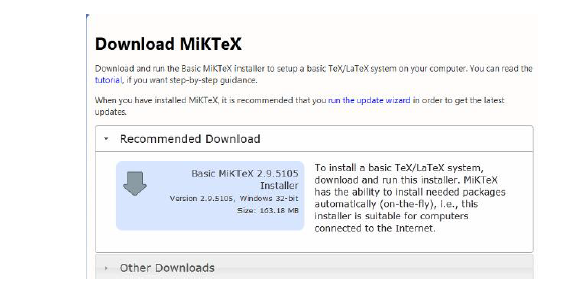
\includegraphics[width =10 cm]{img/18.png}
	\captionof{figure}{Download MikTeX}
	\label{picture label}
\end{center}
\item Setelah software berhasil di download, jalankan software tadi. Akan muncul persetujuan penggunaan MiKTex. Centang {\bf \itshape{I accept the MiKTex copying condition}}, kemudian klik {\bf next}.
\begin{figure}[h!]
    \centering
    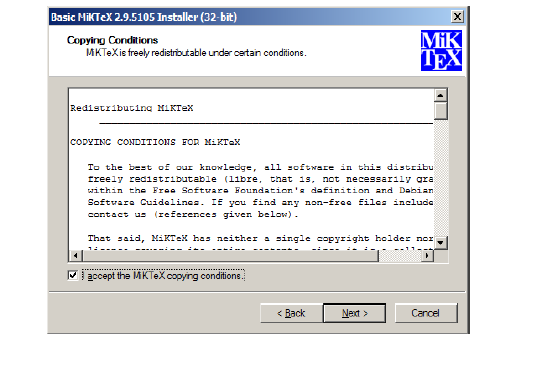
\includegraphics[width =10 cm]{img/19.png}
    \captionof{figure}{MikTeX \textit{pop-up}}
	\label{picture label}
\end{figure}
\newpage
\item Kemudian, akan muncul pilihan untuk siapa saja software ini digunakan. Saran dari penulis klik {\bf Only for nama \itshape User} agar lebih menghemat memory komputer. Kemudian klik {\bf next}.
\begin{figure}[h!]
    \centering
    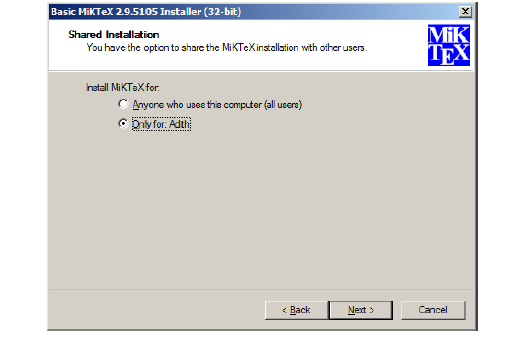
\includegraphics[width =10 cm]{img/20.png}
    \captionof{figure}{MikTeX \textit{pop-up} 2}
	\label{picture label}
\end{figure}
\item Kemudian pilih lokasi untuk penampung software MiKTex. Lalu klik {\bf next}.
\begin{figure}[h!]
    \centering
    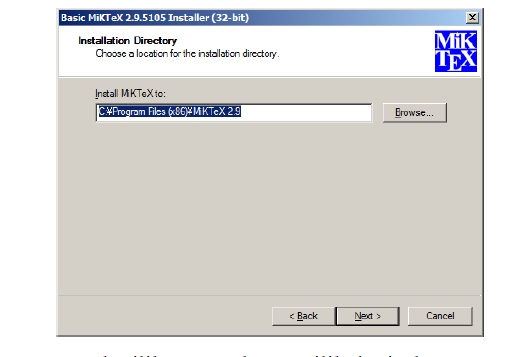
\includegraphics[width =10  cm]{img/21.png}
    \captionof{figure}{MikTeX \textit{pop-up} 3}
	\label{picture label}
\end{figure}
\item Lalu, akan muncul pilihan untuk memilih jenis kertas yang digunakan. Pilih {\bf A4} sebagai jenis kertas dan ask me first. Kemudian klik {\bf next}. Selanjutnya klik {\bf start}.
\newpage
\begin{figure}[h!]
\centering
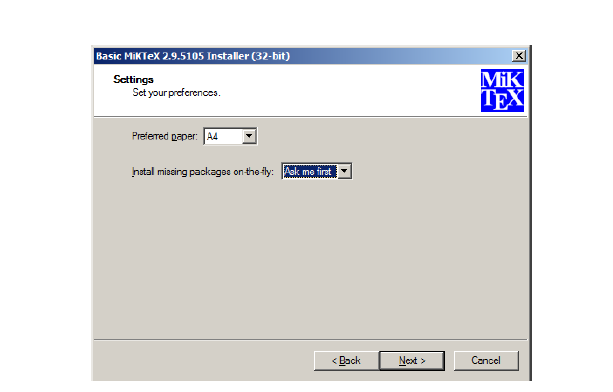
\includegraphics[width =10 cm]{img/22.png}
\end{figure}
\item Tunggu proses instalasi selesai.
\end{enumerate}
LaTex memerlukan teks editor untuk menulis perintah yang akan di eksekusi, serta sebagai compiler dari perintah-perintah tadi. Notepad bawaan windows dapat dijadikan sebagai teks editor. Bila menggunakan notepad, ubah jenis file yang akan disimpan menjadi .tex. Namun untuk para pemula, kami sarankan anda untuk menggunakan software seperti teXstudio, teXworks, ataupun teks editor lainnya yang khusus menangani LaTex. Sebab, software-software tadi menyediakan perintah-perintah yang khusus sehingga memudahkan para pemula untuk belaajr menggunakan LaTex.
\begin{enumerate}
\item {\itshape Download} aplikasi teXstudio di situs {\bf http://texstudio.sourceforge.net/} .
\item Kemudian, klik aplikasi yang telah didownload. Pilih bahasa yang akan digunakan. Kemudian klik {\bf ok}.
\begin{figure}[h!]
\centering
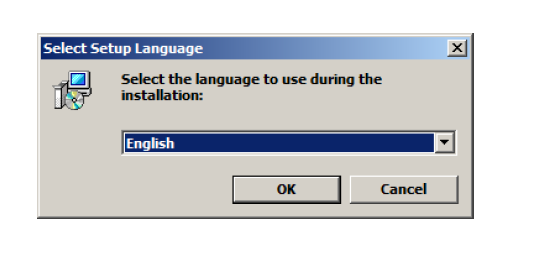
\includegraphics[width =10 cm]{img/23.png}
\end{figure}
\newpage
\item Klik {\bf next} untuk melanjutkan ke proses berikutnya.
\begin{figure}[h!]
\centering
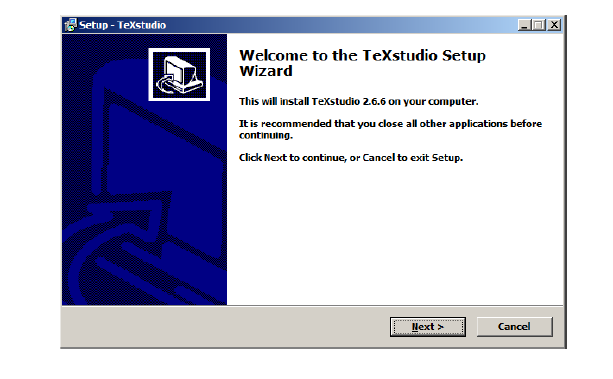
\includegraphics[width =10 cm]{img/24.png}
\end{figure}
\item Klik {\bf browse} untuk memilih lokasi file teXstudio. Setelah memilih lokasinya, klik {\bf next}.
\begin{figure}[h!]
\centering
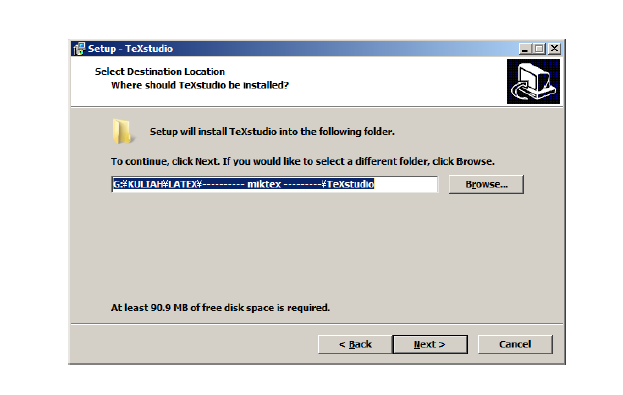
\includegraphics[width =10 cm]{img/25.png}
\end{figure}
\newpage
\item Kemudian akan muncul pilihan untuk memilih tempat folder. Klik {\bf next} untuk melanjutkan proses.
\begin{figure}[h!]
\centering
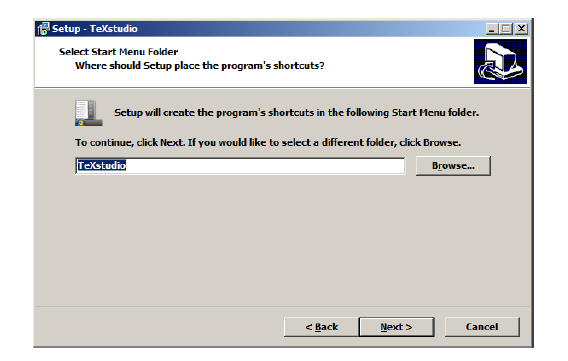
\includegraphics[width =10 cm]{img/26.png}
\end{figure}
\item Klik {\bf install} untuk memulai proses instalasi.
\newpage
\begin{figure}[h!]
\centering
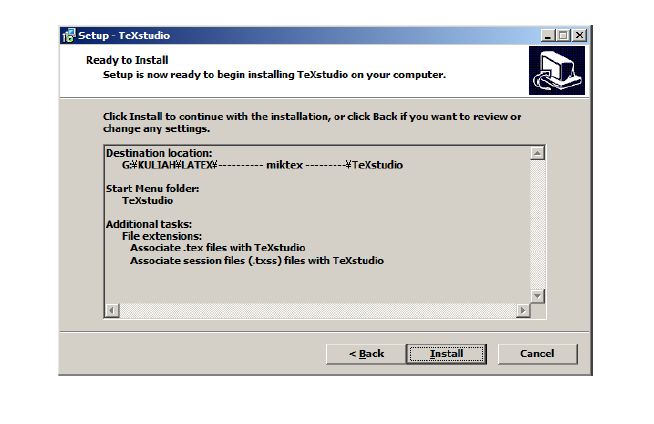
\includegraphics[width =10cm]{img/27.png}
\end{figure}
\item Tunggu proses instalasi selesai.
\end{enumerate}
\section{Perintah-Perintah Dalam  Latex}
\subsection{Format Perintah}
\begin{raggedleft}
Semua perintah Latex diawali dengan tanda backslash (\textbackslash). Tanda ini memberitahukan kepada LATEX untuk melakukan hal tertentu pada bagian dokumen tersebut. Perintah-perintah dalam Latex biasanya sudah cukup menjelaskan apa yang akan dilakukan LATEX pada dokumen kita. Misalnya:\end{raggedleft}
\begin{table}[h!]
\begin{tabular}{ll p{5 cm}}
\bfseries{\textcolor{blue}{\textbackslash tableofcontents}} &:& perintah ini digunakan untuk menambahkan daftar isi sebuah   dokumen.\\
\bfseries{\textcolor{blue}{\textbackslash documentclass}} & :& perintah untuk menentukan jenis dokumen yang akan dibuat  dan harus ada pada awal  dokumen. \\
\bfseries{\textcolor{blue}{\textbackslash bfseries}}&:& perintah untuk menebalkan teks pada dokumen Latex
\end{tabular}
\end{table}
\subsection{Preamble, Dekalarasi \& Environment}
\begin{raggedleft}Yang dimaksud dengan preamble/pembukaan adalah bagian dari dokumen LATEX di antara per-intah \textbackslash  documentclass dan perintah \textbackslash begin{document}. Hanya ada beberapa perintah yang hanya bisa diletakkan di bagian ini. Yang paling umum diletakkan dalam bagian preamble adalah deklarasi penggunaan paket-paket LATEX .\end{raggedleft}
\subsection{Spasi dalam Latex}
\begin{raggedleft}Dalam dokumen LATEX semua baris-baris kosong, spasi yang banyak, dan tabulasi dianggap sebagai 1 spasi atau 1 baris kosong saja selama proses pengaturan tulisan. LATEX mengatur spasi dan perataan teks (alignment) berdasarkan perintah yang diterimanya, sehingga kita mampu mengaturnya secara tepat. Contohnya :\end{raggedleft}
\begin{table}[h!]
\begin{tabular}{|p{5 cm} p{8 cm}|}
\hline
\bfseries{\textcolor{blue}{\textbackslash chapter}}\bfseries{\textcolor{red}{ \{}}Pendahuluan\bfseries{\textcolor{red}{\}}}& \\
ini adalah contoh dokumen &  \\
\hline
\end{tabular}
\end{table}
\\ \begin{raggedleft}Format penulisan di atas akan menghasilkan keluaran yang sama jika dituliskan seperti ini : \end{raggedleft}
\begin{table}[h!]
\begin{tabular}{|p{13.5 cm}|}
\hline
\bfseries{\textcolor{blue}{\textbackslash chapter}}  \bfseries{\textcolor{red}{\{}}Pendahuluan\bfseries{\textcolor{red}{\}}} ini adalah contoh dokumen \\
\hline
\end{tabular}
\end{table}
\\
Ada perintah khusus untuk membuat spasi dengan panjang tertentu baik secara horizontal maupun vertikal, yaitu :
\begin{itemize}
\item Jika kita ingin membuat jarak dengan panjang tertentu antara 2 baris, kita dapat menggunakan tanda ‘ \textbackslash \textbackslash’ di akhir baris. Kita juga dapat menentukan sendiri panjang baris kosong dengan menggunakan perintah seperti contoh berikut ini : 
\begin{table}[h!]
\begin{tabular}{|p{13.5 cm}|}
\hline
\bfseries{\textcolor{red}{baris 1}} \textbackslash  \textbackslash  \\
\bfseries{\textcolor{blue}{\textbackslash vspace \{ }} \bfseries{\textcolor{red}{2 cm}} \textcolor{blue}{ \} } \\
\bfseries{\textcolor{red}{baris 2}} \textbackslash  \textbackslash  \\
\hline
\end{tabular}
\end{table}
\\
Dengan perintah ini LATEX akan membuat mengosongkan baris-baris sepanjang 2 centimeter.Tanpa perintah ini sejauh apapun kita membuat spasi dalam teks dokumen, LATEX akan tetap menganggapnya 1 spasi.
\item Jika kita ingin membuat spasi sejauh beberapa centimeter antara 2 kata dibutuhkan
perintah : \\
\begin{table}[h!]
\begin{tabular}{|p{13.5 cm}|}
\hline
kata 1 \textbackslash hspace\{2cm\} kata 2\\
\hline
\end{tabular}
\end{table}
\\
Dengan perintah ini LATEX akan membuat spasi sejauh 2 centimeter. Sama seperti poin sebelumnya tanpa perintah ini sejauh kita membuat spasi dalam teks dokumen, LATEX akan tetap menganggapnya 1 spasi. \\[0.5 cm]

Jadi secara umum aturan yang dapat dipakai adalah : akhiri paragraf dengan tanda ‘\textbackslash \textbackslash’ dan berikan 1 baris kosong antara tiap-tiap paragraf dan 1 spasi kosong antara masing-masing kata.

\end{itemize}
\subsection{Hyphenation}
hyphenation berfungsi untuk memperbaiki pemenggalan kata yang mungkin kurang tepat, sebagai contohnya  kata “mungkin” dipenggal menjadi kata “mun-gkin”. Berikut adalah contoh penggunaan hyphenation: \\[0.5 cm]
\begin{tabular}{|p{13.5 cm}|}
\hline
\textbackslash usepackage \{hyphenation\} \\
          \textbackslash hyphenation \{mung-kin, sa-ngar, mi-num\}\\

\hline
\end{tabular}
\subsection{Alignment}
Alignmen atau yang disebut dengan perataan baris pada Latex dibagi menjadi 3 jenis yaitu: rata kiri, rata, rata kanan, dan rata tengah. Dokumen pada Latex secara default diatur dengan perataan justified (rata kanan kiri). Berikut adalah contoh penggunaan alignmen pada Latex:
\begin{description}
\item[a.]	Alignment rata kiri\\
\begin{tabular}{|p{12cm}|}
\hline
\textbackslash begin\{raggedright\} \\
    Isi dokumen diatur secara rata kiri \\
  \textbackslash end\{raggedright\} \\
\hline
\end{tabular}
\item[b.] Alignment rata kanan\\
\begin{tabular}{|p{12cm}|}
\hline
\textbackslash begin\{raggedleft\} \\
    Isi dokumen diatur secara rata kanan \\
  \textbackslash end\{raggedleft\} \\
\hline
\end{tabular}
\item[c.]  Alignment  rata tengah\\
\begin{tabular}{|p{12cm}|}
\hline
\textbackslash begin\{center\} \\
    Isi dokumen diatur secara rata tengah \\
  \textbackslash end\{center\} \\
\hline
\end{tabular}
\end{description}
\subsection{Bahasa}
\begin{raggedleft} LATEX dapat mengatur tulisan mengikuti aturan ejaan yang dimiliki beberapa bahasa tertentu. Kemampuan ini diatur oleh babel package yang dimiliki LATEXH˙ al tersebut berpengaruh pada pemenggalan kata, spasi setiap kata, indentasi, dan beberapa judul bagian dokumen yang digunakan dalam heading. Mengubah pengaturan bahasa dengan menggunakan babel akan secara otomatis mengubah nama-nama dari unit struktur dokumen (seperti misalnya Abstract, Chapter, Index) menjadi terjemahannya.\end{raggedleft} \\[0.5 cm]

\begin{raggedleft} Perintah yang mengatur LATEX untuk menggunakan babel bahasa Indonesia adalah seperti berikut ini :\end{raggedleft} \\
\begin{tabular}{|p{13.5cm}|}
\hline
\textbackslash documentclass [a4paper, 12pt]\{report\}\\
\textbackslash usepackage[bahasa]\{babel\}\\
Cara mengatur\\
\textbackslash begin\{document\} bahasa\\
. . . . . . . . . . . . . . . . . .\\
. . . . . . . . . . . . . . . . . .\\
\textbackslash end\{document\}\\
\hline
\end{tabular}
\subsection{Keterangan}
Jika ini menambahkan keterangan pada dokumen Latex (yang tidak akan tercetak). Caranya adalah dengan menambahkan  tanda \textquotedblright \%\textquotedblleft  di awal kata yang akan dijadikan keterangan. Contohnya:\\[0.5 cm]
\begin{tabular}{|p{13.5cm}|}
\hline
 \textbackslash documentclass [a4paper, 12pt]\{report\} \% untuk menentuka ukuran kertas dan huruf\\
\textbackslash  usepackage[bahasa]\{babel\} \% untuk merubah kata kedalam bahasa Indonesia.\\
\textbackslash  begin\{document\}
   \% ini adalah baris keterangan, baris ini tidak akan tercetak pada saat file dijalankan\\
  ……………….
\textbackslash end\{document\}\\

\hline
\end{tabular}
\subsection{Karakter Khusus}
Ada beberapa karakter tertentu yang membutuhkan perintah khusus untuk menuliskannya pada dokumen Latex. Berikut adalah diantaranya:
\begin{longtable}{|l|l|l|l|}
\hline
Karakter&Penulisan&Karakter&Penulisan\\ \hline
\textbackslash & \textbackslash textbackslash& \$ &\textbackslash \$\\ \hline
\%&\textbackslash\%&\^{} & \textbackslash \^{}\{\}\\ \hline
\_&\textbackslash\_&\~{}&\textbackslash \~{}\{\}\\ \hline
\{&\textbackslash\{&\}&\textbackslash\}\\ \hline
\textgreater&\textbackslash textgreater&\textless &\textbackslash textless\\ \hline
\textbar&\textbar& \textquotedblleft& \textbackslash textquotedblleft\\ \hline
\textquotedblright&\textbackslash textquotedblright & \textquoteleft&\textbackslash textquoteleft\\ \hline
\textquoteright&\textbackslash textquoteright&\#& \textbackslash \#\\ \hline
\end{longtable}

\begin{raggedleft} Dalam bahasa asing sering digunakan aksen dan symbol-simbol tertentu dalam penulisan bahasanya. Berikut adalah beberapa aksen dan symbol yang sering digunakannya:\end{raggedleft} \\
\begin{figure}[h!]
\centering
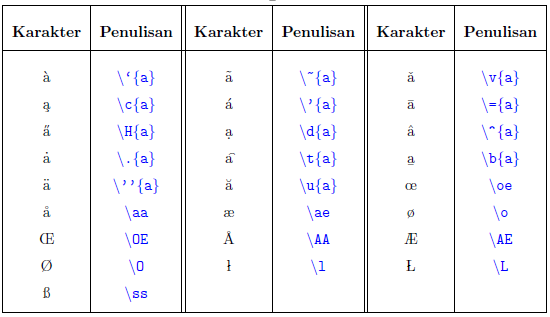
\includegraphics[width = 10cm]{img/1.png}
\end{figure}
\subsection{Font dalam Latex}
\subsubsection{Jenis Font}
Font standar dalam Latex yang disediakan ada 3 jenis yaitu:
\begin{enumerate}
\item Roman, berikut adalah cara menggunakan jenis font di bawah ini:\\
\begin{tabular}{|p{12 cm }|}
\hline
\{ \textbackslash rmfamily teks yang akan diformat\}\\
\hline
\end{tabular}
\item Sans serif, berikut adalah cara menggunakan jenis font di bawah ini:\\
\begin{tabular}{|p{12 cm }|}
\hline
\{ \textbackslash sffamily teks yang akan diformat\}\\
\hline
\end{tabular}
\item Typewriter, berikut adalah cara menggunakan jenis font di bawah ini:\\
\begin{tabular}{|p{12 cm }|}
\hline
\{ \textbackslash ttfamily teks yang akan diformat\}\\
\hline
\end{tabular}
\end{enumerate}
\subsubsection{Bentuk Font}
Bentuk font yang disediakan pada Latex, yaitu:
\begin{enumerate}
\item Italic, cara mengatur bentuk font seperti ini adalah:\\
\begin{tabular}{|p{12 cm }|}
\hline
\{\textbackslash itshape teks yang akan diformat\}\\
\hline
\end{tabular}

\item Slanted,  cara mengatur bentuk font seperti ini adalah:\\
\begin{tabular}{|p{12 cm }|}
\hline
\{\textbackslash slshape teks yang akan diformat\}\\
\hline
\end{tabular}
\item 	Vertical, Cara mengatur bentuk font seperti ini adalah:\\
\begin{tabular}{|p{12 cm }|}
\hline
\{\textbackslash upshape teks yang akan diformat\}\\
\hline
\end{tabular}
\item   Small Caps, cara mengatur bentuk font seperti ini adalah:\\
\begin{tabular}{|p{12 cm }|}
\hline
\{\textbackslash scshape teks yang akan diformat\}\\
\hline
\end{tabular}
\end{enumerate}
\subsubsection{Ukuran Font}
Ada beberapa macam ukuran font yang ada dalam dokumen Latex yaitu:
\begin{figure}[h!]
\centering

\includegraphics[width=  10 cm]{img/2.png}
\end{figure}
\\
Berikut cara menggunakan ukuran-ukuran font tersebut adalah:
\begin{description}
\item[-]Tiny : \{\textbackslash tiny teks yang akan diformat\}
\item[-] Scriptsize : \{\textbackslash scriptsize teks yang akan diformat\}
\item[-] Footnotesize : \{\textbackslash  footnotesize  teks yang akan diformat\}
\item[-] Small : \{\textbackslash small teks yang akan diformat\}
\item[-] Normal :  \{\textbackslash normal teks yang akan diformat\}
\item[-] Large :  \{\textbackslash large teks yang akan diformat\}
\item[-] Larger :  \{\textbackslash Large teks yang akan diformat\}
\item[-] Largest : \{\textbackslash LARGE teks yang akan diformat\}
\item[-] Huge :  \{\textbackslash huge teks yang akan diformat\}
\item[-] Huger :  \{\textbackslash Huge teks yang akan diformat\}
\end{description}
\subsection{Mode Verbatim}
\begin{raggedleft}Mode verbatim berfungsi untuk menampilkan sesuai teks seperti apa yang kita ketik. Pada dasarnya semua dokumen Latex yang ingin ditampilkan pada file keluarannya harus dilengkapi dengan perintah. Untuk menampilkan teks keluaran sesuai apa yang kita ketik maka gunakan mode verbatim.\end{raggedleft}
\vspace{0.5 cm}

\begin{raggedleft}Contoh penulisan tanpa menggunkana mode verbatim:\end{raggedleft}\\
\begin{tabular}{|p{13.5 cm}|}
\hline
Ini adalah baris pertama \\[0.5 cm]


Ini adalah baris kedua     \hspace{0.5 cm}   dari contoh\\
\hline
\end{tabular}\\[0.5 cm]
\vspace{0.5 cm}
Hasil outputnya:\\
\begin{tabular}{|p{13.5 cm}|}
\hline
Ini adalah baris pertama \\


Ini adalah baris kedua  dari contoh\\
\hline
\end{tabular}\vspace{0.5 cm}
\begin{raggedleft}
Pada contoh di atas terlihat seberapa jauhpun kita membuat spasi horizontal atau vertical, hasilnya tidak akan terpengaruh. Hasilnya hanya menampilkan sesuai yang diperintahkan dan menurut standar Latex. Supaya teks yang dihasilkan sama persis susunan dan formasinya seperti apa yang kita ketik, kita bisa menggunakan mode verbatim. Berikut adalah cara penggunaanya:\end{raggedleft} \\[0.5 cm]
\begin{tabular}{|p{13.5 cm}|}
\hline
\textbackslash begin \{verbatim\}\\
Ini adalah baris pertama \\[0.5 cm]


Ini adalah baris kedua     \hspace{0.5 cm}   dari contoh\\
\textbackslash end\{verbatim\} \\
\hline
\end{tabular}\\[0.5 cm]
Hasil outputnya: \\[0.5 cm]
\vspace{0.5 cm}
\begin{tabular}{|p{13.5 cm}|}
\hline
\begin {verbatim}
Ini adalah baris pertama 


Ini adalah baris kedua      dari contoh
\end{verbatim} \\
\hline
\end{tabular}\\[0.5 cm]
Mode verbatim ini sangat cocok digunakan untuk penulisan source code atau dokumentasi pembuatan perangkat lunak.
\section{Struktur Dokumen Latex}
\subsection{Document Class}
Class file pada LATEX menentukan layout halaman, jenis heading, dan berbagai perintah dan environment yang diperlukan untuk mengatur style dokumen. Cara untuk mendeklarasikan Document Class adalah memulai dokumen dengan :\\[0.5 cm]
\begin{tabular}{|p{13.5 cm}|}
\hline
\textbackslash documentclass\{class\}\\
\hline
\end{tabular}\\[0.5 cm]
Ada beberapa jenis document class yang bisa dipakai dalam sebuah dokumen, yaitu :
\begin{itemize}
\item {\bf report} : kelas ini dapat digunakan untuk membuat laporan (report) baik dalam bidang
bisnis, teknik, hukum, akademis, atau ilmu pengetahuan.
\item  {\bf article} : kelas ini dapat digunakan untuk membuat paper, artikel sebuah jurnal atau
majalah, review, paper untuk konferensi, atau catatan riset.
\item {\bf book} : kelas ini digunakan untuk membuat buku dan thesis.
\item {\bf letter} : kelas ini digunakan untuk membuat surat.
\end{itemize}
Biasanya kelas ‘article’ adalah yang paling sering digunakan untuk sembarang jenis dokumen. Masing-masing kelas di atas memiliki strukturnya sendiri. Misalnya pada kelas article tidak ada elemen bab, tidak seperti pada kelas report dan book.\\[0.5 cm]
\vspace{0.5 cm}
Secara sederhana struktur dokumen  Latex adalah sebagai berikut:\\
\begin{tabular}{|p{13.5 cm}|}
\hline
\textbackslash documentclass\{. . .\}\\
\textbackslash begin\{document\}\\
      Bagian isi dokumen\\
\textbackslash end\{document\}\\
\hline
\end{tabular}
\subsection{Document Class Option}
Document Class Option maksudnya adalah pilihan yang tersedia pada kelas dokumen yang bisa kita tentukan sendiri isinya. Opsi pada suatu kelas dokumen dituliskan seperti berikut :\\[0.5 cm]
\begin{tabular}{|p{13.5 cm}|}
\hline
          \textbackslash documentclass [ option1, option2 ] \{ class \}\\
\hline
\end{tabular}\\[0.5 cm]
Seperti terlihat di atas, kita dapat menentukan beberapa opsi sekaligus dalam tanda kurung dengan dibatasi tanda koma.\\[0.5 cm]

\begin{raggedleft}Default opsi yang digunakan oleh LATEX antara lain :\end{raggedleft}

\begin{itemize}
\item Ukuran kertas yang digunakan adalah A4.
\item Ukuran font yang digunakan adalah 10pt untuk semua kelas dokumen.
\item Layout halaman yang digunakan adalah two-sided printing khusus untuk kelas book dan report, dan one-sided printing khusus untuk kelas article dan letter.
\item  Halaman judul yang terpisah di bagian awal dokumen khusus untuk kelas book dan
report.
\end{itemize}
Opsi di atas dapat modifikasi dengan beberapa opsi berikut :
\begin{itemize}
\item Ukuran kertas : Kita dapat menentukan sendiri ukuran kertasnya. Cara penulisannya:\\[0.5 cm]
\begin{tabular}{|p{12 cm}|}
\hline
\textbackslash documentclass [ a3paper ] \{ class \} atau \\
\textbackslash documentclass [ letterpaper ] \{ class \}\\
\hline
\end{tabular}
\item Ukuran font : kita dapat memilih ukuran 10pt, 11pt, atau 12pt. Cara penulisannya :\\[0.5 cm]
 \begin{tabular}{|p{12 cm}|}
\hline
\textbackslash documentclass [ a4paper, 11pt ] \{class\}\\
\hline
\end{tabular}\\[0.5 cm]
Setelah kita menentukan ukuran font yang dipakai, semua font dalam dokumen akan diatur sedemikan sehingga memiliki ukuran sesuai dengan yang kita tentukan. Font yang dipakai pada header, footer disesuaikan secara proporsional dengan ukuran font tersebut.
\item Layout halaman dapat kita tentukan sendiri dengan 2 pilihan berikut :
\begin{itemize}
\item[-] oneside : jika kita menginginkan layout one-sided printing saat menggunakan kelas book dan report.
\item[-] twoside : jika kita menginginkan layout two-sided printing saat menggunakan kelas  article.
\item[-] titlepage : jika kita menginginkan kelas article untuk memiliki halaman judul yang          terpisah di bagian awal dokumen.
\item[-]draft : opsi ini mengatur LATEX supaya menandai masalah-masalah yang timbul seperti masalah pemenggalan kata (pemenggalan kata tidak tepat) atau masalah perataan tulisan (ada baris tertentu yang melebihi batas kanan dokumen). Tanda yang akan digunakan LATEX adalah sebuah persegi kecil di bagian kanan dokumen tempat terjadinya masalah.
\end{itemize}
\end{itemize}
\section{Paket (Package)}
Yang dimaksud dengan paket dalam LATEX adalah fungsi-fungsi yang dipakai untuk menambah kemampuan LATEX melakukan pengaturan dokumen. Ada banyak sekali paket yang dimiliki LATEX baik yang sudah terintegrasi bersamaan di dalam instaler LATEX maupun yang belum. Paket-paket yang belum terinstal bisa didownload dari http://www.ctan.org. Untuk menggunakan paket tertentu dalam dokumen yang kita buat, kita perlu mendeklarasikannya terlebih dulu pada bagian preamble1. Cara menggunakan paket yang sudah tersedia/terintegrasi di dalam LATEX adalah seperti ini :\\[0.5 cm]
\begin{tabular}{|p{13.5 cm}|}
\hline
\textbackslash documentclass \{class\}\\
\textbackslash usepackage [ option ] \{nama paket\}\\\
\textbackslash begin\{document\}\\
. . . . . . . . . . . . . . . . . .\\
. . . . . . . . . . . . . . . . . .\\
. . . . . . . . . . . . . . . . . .\\
\textbackslash end\{document\}\\
\hline

\end{tabular}\\[0.5 cm]
Beberapa paket yang terintegrasi dalam LATEX antara lain :
\begin{enumerate}
\item	graphicx : paket ini membuat LATEX mampu menghasilkan gambar grafis dan juga membuat LATEX mampu menampilkan gambar yang kita sertakan dalam dokumen.
\item	hyperref : paket ini membuat LATEX mampu menghasilkan dokumen yang memiliki dynamic link2 ke alamat tertentu.
\item babel : paket ini membuat LATEX mampu mengenali format bahasa yang digunakan
\item	seperti yang sudah dijelaskan pada subbab Bahasa di Bab Perintah-Perintah LATEX .
\item	color : paket ini membuat LATEX mampu menghasilkan teks dokumen yang memiliki warna sesuai warna yang ditentukan.
\item	makeidx : paket ini membuat LATEX mampu menghasilkan indeks dari dokumen yang dibuat.
\end{enumerate}
\section{Document Enviroment}
Yang dimaksud dengan document environment adalah bagian dalam sebuah dokumen LATEX dimana isi sebenarnya dari dokumen itu sendiri ditempatkan.\\[0.5 cm]
\begin{tabular}{|p{13.5 cm}|}
\hline
\textbackslash documentclass\{class\}\\
\textbackslash begin\{document\}\\\
. . . . . . . . . . . . . . . . . .\\
. . . . . . . . . . . . . . . . . .\\
. . . . . . . . . . . . . . . . . .\\
\textbackslash end\{document\}\\
\hline

\end{tabular}\\[0.5 cm]
Semua teks isi dari dokumen harus dituliskan di bagian titik-titik tersebut di atas. Teks yang ditulis sebelum \textbackslash begin\{document\} dan sesudah \textbackslash end\{document\}, kelak tidak akan muncul pada dokumen hasil compile. Struktur \textbackslash begin . . . \textbackslash end inilah yang disebut dengan environment. Environment membatasi bagian teks yang akan diatur dengan aturan tertentu. Bagian antara deklarasi kelas dokumen dengan awal document environment disebut preamble.
\section{Penulisan Judul}
Judul dalam sebuah dokumen latex diletakan pada awal document environment, Cara penulisannya sebagai berikut:\\[0.5 cm]
\begin{tabular}{|p{13.5 cm}|}
\hline
\textbackslash documentclass [a4paper, 12pt]\{report\}\\
\textbackslash begin\{decument\}\\
        \textbackslash titile\{Judul Document\}\\
        \textbackslash autor\{Nama Penulis\}\\
        \textbackslash date\{Tanggal Pembuatan\}\\
        \textbackslash maketitle\\
. . . . . . . . . . . . . . . .\\
. . . . . . . . . . . . . . . . \\
\textbackslash end\{document\}\\

\hline

\end{tabular}\\[0.5 cm]
\section{Abstrak}
Pada dokumen kelas article dan report umumnya memiliki abstrak/ringkasan. Latex memiliki cara khusus untuk menuliskan abstrak. Berikut adalah cara penulisannya:\\
\begin{tabular}{|p{13.5 cm}|}
\hline
 \textbackslash  documentclass [a4paper, 12pt]\{report\}\\
 \textbackslash  begin\{decument\} \\
         \textbackslash  titile\{Judul Document\} \\
         \textbackslash  autor\{Nama Penulis\} \\
         \textbackslash  date\{Tanggal Pembuatan\}\\
         \textbackslash maketitle \\

         \textbackslash begin\{abstract\}\\
             Isi abstrak\\
         \textbackslash end\{abstract\}\\
. . . . . . . . . . . . . . . . \\
\textbackslash end\{document\}\\

\hline

\end{tabular}\\[0.5 cm]
\begin{raggedleft}Jika ingin mengubah judul abstrak digunakan perintah ini sebelum \end{raggedleft}\\  \textbackslash begin\{abstract\}:\\[0.5 cm]
\begin{tabular}{|p{13.5 cm}|}
\hline
\textbackslash renewcommand\{\textbackslash abstractname\}\{RINGKASAN LAPORAN\}\\
\hline
\end{tabular}\\[0.5 cm]
Perintah di atas akan mengganti judul abstrak menjadi \textquotedblleft RINGKASAN LAPORAN \textquotedblright
\section{Sistematika Isi Dokumen}
\begin{raggedleft} LATEX memiliki kemampuan untuk membagi dokumen dalam suatu susunan struktural (bab, subbab, subsubbab, dst) sampai 7 tingkatan. Berikut adalah daftar struktur yang disediakan dalam latex:\end{raggedleft}\\[0.5 cm]
\begin{tabular}{|p{10 cm}|p{3.5 cm}|}
\hline
Struktur&Perintah\\ \hline
Bagian (Part)&\textbackslash part\{...\}\\
Bab (Chapter)&\textbackslash chapter\{...\}\\
Subbab (Section)&\textbackslash section\{...\}\\
Subsubbab (subsubsection)&\textbackslash subsection\{...\}\\
Subsubsubbab (subsubsection)&\textbackslash subsubsection\{...\}\\
Paragraf berjudul (titled paragraph)&\textbackslash paragraph\{...\}\\
Anak paragraph berjudul (titled subparagraph)&\textbackslash subparagraph\{...\}\\
\hline
\end{tabular}\\[0.5 cm]
Ada beberapa hal yang perlu diketahui tentang penggunaan struktur di atas :\\
\begin{itemize}
\item Hanya dokumen dengan kelas book dan report bisa menggunakan semua struktur di atas.
\item  Dokumen kelas article hanya bisa menggunakan kelas \textbackslash section\{...\} dan struktur di bawahnya bawah.
\item  Dokumen kelas letter tidak dapat menggunakan semua struktur di atas.
\end{itemize}
Contoh penggunaanya adalah sebagai berikut:\\
\begin{tabular}{|p{13.5 cm}|}
\hline
\textbackslash documentclass [a4paper, 12pt] \{report\}\\
\textbackslash begin\{document\}\\
   \textbackslash title\{Judul Dokumen\}\\
    \textbackslash author\{Nama Penulis\}\\
    \textbackslash date\{Tanggal Pembuatan\}\\
    \textbackslash maketitle\\

       \textbackslash begin\{abstract\}\\
          isi abstract\\
       \textbackslash end\{abstract\}\\

        \textbackslash chapter\{Pendahuluan\}\\
           isi bab I pendahuluan\\
         \textbackslash section\{Latar Belakang\}\\
           isi subbab latar belakang\\

          \textbackslash chapter\{Dasar Teori\}\\
              isi bab II dasar teori\\
          \textbackslash section\{Tinjauan Pustaka\}\\
              isi subbab tinjauan pustaka\\

\textbackslash end\{document\}\\
\hline
\end{tabular}
\section{Daftar Berurut }
Ada 3 Jenis cara penulisan daftar berurut yaitu:
\begin{enumerate}
\item Daftar dengan penomoran menggunakan simbol (Bulleted List), contohnya seperti
berikut ini :
\begin{itemize}
\item Apel
\item Jeruk 
\item Semangka
\item Durian
\end{itemize}
Format penulisan daftar seperti ini adalah sebagai berikut :\\[0.5 cm]
\begin{tabular}{|p{12.5 cm}|}
\hline
\textbackslash begin\{itemize\}\\
\textbackslash item . . .\\
\textbackslash item . . .\\
\textbackslash item . . .\\
. . . .\\
\textbackslash end\{itemize\}\\

\hline
\end{tabular}\\[0.5 cm]
Isi daftar dituliskan setelah \textbackslash item. Simbol yang dipakai dapat kita tentukan sendiri.
Sebagai contoh jika kita ingin menggunakan tanda * sebagai penanda item, caranya adalah dengan menambahkan keterangan simbol yang digunakan seperti berikut : \textbackslash item[*] ...
\item Daftar dengan penomoran menggunakan angka (Numbered List), contohnya seperti berikut ini :\\
\begin{enumerate}
\setlength{\itemindent}{-0.1 in}
\setlength\itemsep{0 em}
\item[1.] Apel
\item[2.] Jeruk 
\item[3.] Semangka
\item[4.] Durian
\end{enumerate}
Format penulisan daftar seperti ini adalah sebagai berikut :\\[0.5 cm]
\begin{tabular}{|p{12.5 cm}|}
\hline
\textbackslash begin\{enumerate\}\\
\textbackslash item . . .\\
\textbackslash item . . .\\
\textbackslash item . . .\\
. . . .\\
. . . .\\
\textbackslash end\{enumerate\}\\

\hline
\end{tabular}
\item Daftar deskripsi, contohnya seperti berikut ini :
\begin{description}
\item[ITB]Institut Teknologi Bandung
\item[UI]Universitas Indonesia
\item[IPB]Institut Pertanian Bogor
\item[UGM]Universitas Gajah Mada
\end{description}
Cara penulisannya adalah seperti berikut ini :\\[0.5 cm]
\begin{tabular}{|p{12.5 cm}|}
\hline
\textbackslash begin\{description\}\\
\textbackslash item[ Hal 1 ] penjelasan hal 1\\
\textbackslash item[ Hal 2 ] penjelasan hal 2\\
\textbackslash item[ Hal 3 ] penjelasan hal 3\\
\textbackslash item[ Hal 4 ] penjelasan hal 4\\
. . . .\\
. . . .\\
\textbackslash end\{description\}\\

\hline
\end{tabular}
\end{enumerate}
\section{Daftar isi}
Untuk menampilkan daftar isi digunakan perintah :\\[0.5 cm]

\textbackslash tableofcontents\\[0.5 cm]


\begin{raggedleft}Perintah ini diletakkan pada bagian dimana daftar isi tersebut akan ditempatkan. Biasanya daftar isi ditempatkan tepat setelah abstrak/kata pengantar.\end{raggedleft}\\[0.5 cm]


\begin{raggedleft} Untuk menampilkan daftar gambar digunakan perintah :\end{raggedleft}\\[0.5 cm]



\textbackslash listoffigures \\[0.5 cm]


\begin{raggedleft} Untuk menampilkan daftar tabel digunakan perintah :\end{raggedleft}\\[0.5 cm]



\textbackslash listoftables\\[0.5 cm]


\begin{raggedleft} LATEX menghasilkan file berekstensi *.toc untuk menangani daftar isi, daftar gambar, dan daftar tabel. Jika daftar isi, daftar gambar, dan daftar tabel tidak menampilkan keseluruhan struktur dokumen dengan benar, kita dapat mengatur sendiri isinya dengan cara menambahkan perintah-perintah berikut :\end{raggedleft}\\[0.5 cm]



\textbackslash addcontentsline\{toc\}\{struktur\}\{teks yang ingin ditampilkan pada daftar isi\}\\[0.5 cm]


\begin{raggedleft} Struktur dapat diisi dengan chapter, section, subsection, dst, tergantung bagian dokumen yang ingin kita masukkan ke dalam daftar isi. Dengan perintah di atas LATEX akan menghasilkan baris baru dalam daftar isi dan akan secara otomatis menentukan nomor halaman bagian tersebut.\end{raggedleft}
\section{Tabel}
\subsection{Tabel}
Untuk menempatkan sebuah tabel dalam dokumen LATEX caranya adalah menggunakan table environment :\\[0.5 cm]
\begin{tabular}{|p{13.5 cm}|}
\hline
\textbackslash begin\{table\}\\
...\\
\textbackslash end\{table\}\\
\hline
\end{tabular}\\[0.5 cm]
Bagian titik-titik tersebut adalah bagian isi dari tabel itu sendiri. Cara mengisi bagian tersebut adalah seperti berikut :\\[0.5 cm]
\begin{tabular}{|p{13.5 cm}|}
\hline
\textbackslash begin\{center\} 
\textbackslash begin\{tabular\}\{\textbar c\textbar l\textbar r\textbar\}
\textbackslash hline\\
Judul Kolom 1 \& Judul Kolom 2 \& Judul Kolom 3 \\
\textbackslash hline\\
Isi Baris 1 Kolom 1 \& Isi Baris 1 Kolom 2 \& Isi Baris 1 Kolom 3 \\
Isi Baris 2 Kolom 1 \& Isi Baris 2 Kolom 2 \& Isi Baris 2 Kolom 3 \\
\textbackslash hline\\
\textbackslash end\{tabular\}\\
\textbackslash caption\{Contoh Tabel\}\\
\textbackslash end\{center\}\\
\hline
\end{tabular}\\[0.5 cm]
Hasil dari perintah tersebut adalah sebagai berikut :\\[0.5 cm]
\begin{center} 
\begin{tabular}{|c|l|r|}
\hline
Judul Kolom 1 & Judul Kolom 2 & Judul Kolom 3 \\
\hline
Isi Baris 1 Kolom 1 & Isi Baris 1 Kolom 2 & Isi Baris 1 Kolom 3 \\
Isi Baris 2 Kolom 1 & Isi Baris 2 Kolom 2 & Isi Baris 2 Kolom 3 \\
\hline
\end{tabular}

\end{center}
Ada beberapa hal yang perlu diketahui dari format perintah tersebut di atas :\\
\begin{itemize}
\item {\textbar c\textbar l\textbar r\textbar} adalah bagian yang menentukan banyaknya kolom yang akan dihasilkan.    Huruf huruf tersebut mewakili center, left, \& right, yaitu menentukan alignment dari isi sel yang dibuat. Sementara garis — menentukan apakah tabel ingin dibatasi garis atau tidak. Jika antara kolom maupun tidak ingin diberi garis batas, kita tinggal menghilangkan — tersebut.
\item  Pengaturan posisi tabel dapat kita tentukan menurut 2 hal :
\begin{itemize}
	  \item[-] Perataan terhadap tepi dokumen : Dengan mengubah \textbackslash begin\{center\} dan juga
 	     \textbackslash end\{center\} kita bisa menentukan posisi tabel terhadap tepi dokumen.
 	  \item[-] Huruf-huruf pada \textbackslash begin\{table\}[htbp] juga berfungsi sebagai pengatur posisi tabel
                   pada suatu halaman.
\end{itemize}
	\begin{itemize}
	  \item[*] h : tabel diletakkan persis di tempat perintah tersebut dituliskan dalam     dokumen.
	\item[*]  t  : tabel diletakkan di bagian atas halaman.
	\item[*]  b : tabel diletakkan di bagian bawah halaman.
	\item[*]  p : tabel diletakkan pada sebuah halaman khusus yang memuat hanya tabel itu saja.
	\end{itemize}
\item  Untuk menuliskan isi dari masing-masing baris, digunakan format
isi kolom 1 \& isi kolom 2 \& isi kolom 3 dst
Perpindahan kolom saat mengisi sebuah baris ditandai dengan tanda \& .

\item Garis mendatar pada tabel (batas tiap baris) dihasilkan dengan perintah \textbackslash hline
\end{itemize}
\subsection{Long Tabel}
\begin{raggedleft}Long table berfungsi untuk membuat table yang lebih dari satu halaman. Jika anda ingin membuat table dengan isi table yang banyak dan tidak cukup pada satu halaman maka gunakanlah perintah long table.\end{raggedleft}\\

\begin{raggedleft}Berikut adalah cara penggunaan long table dengan menggunakan \end{raggedleft}   \textbackslash usepackage\\ \{longtable\}: \\[0.5 cm]
\begin{tabular}{|p{13.5 cm}|}
\hline
\textbackslash begin\{center\}\\
\textbackslash begin\{longtable\}\{\textbar l\textbar l\textbar l\textbar\}\\
\textbackslash  caption\{contoh table\} \textbackslash\textbackslash \\
    Isi tabel.. \\
    . . . .\\
\textbackslash end\{longtable\}\\
\hline
\end{tabular}\\

\begin{small}
\begin{longtable}[c]{|r|l|r|r|r|l|}
\caption{\textit{Nama tabel}} 
\label{tabel-label}\\
\hline
\multicolumn{1}{|c|}{\textbf{aaa}} &
  \multicolumn{1}{c|}{\textit{\textbf{bbb}}} &
  \multicolumn{1}{c|}{\textbf{ccc}} &
  \multicolumn{1}{c|}{\textbf{ddd}} &
  \multicolumn{1}{c|}{\textbf{eee}} &
  \multicolumn{1}{c|}{\textbf{fff}} \\ \hline
\endhead

1   & Ei utroque electram & 0  & 0  & 10 & Laudem  \\ \hline
2   & Ei utroque electram & 3  & 0  & 7  & Laudem  \\ \hline
3   & Ei utroque electram & 2  & 0  & 8  & Laudem  \\ \hline
4   & Ei utroque electram & 0  & 3  & 7  & Laudem  \\ \hline
5   & Ei utroque electram & 10 & 0  & 0  & Laudem  \\ \hline
6   & Ei utroque electram & 0  & 0  & 10 & Laudem  \\ \hline
7   & Ei utroque electram & 3  & 0  & 7  & Laudem  \\ \hline
8   & Ei utroque electram & 2  & 0  & 8  & Laudem  \\ \hline
9   & Ei utroque electram & 0  & 3  & 7  & Laudem  \\ \hline
10   & Ei utroque electram & 10 & 0  & 0  & Laudem  \\ \hline
11   & Ei utroque electram & 0  & 0  & 10 & Laudem  \\ \hline
12   & Ei utroque electram & 3  & 0  & 7  & Laudem  \\ \hline
13   & Ei utroque electram & 2  & 0  & 8  & Laudem  \\ \hline
14   & Ei utroque electram & 0  & 3  & 7  & Laudem  \\ \hline
15   & Ei utroque electram & 10 & 0  & 0  & Laudem  \\ \hline
16   & Ei utroque electram & 0  & 0  & 10 & Laudem  \\ \hline
17   & Ei utroque electram & 3  & 0  & 7  & Laudem  \\ \hline
18   & Ei utroque electram & 2  & 0  & 8  & Laudem  \\ \hline
19   & Ei utroque electram & 0  & 3  & 7  & Laudem  \\ \hline
20   & Ei utroque electram & 10 & 0  & 0  & Laudem  \\ \hline
21   & Ei utroque electram & 0  & 0  & 10 & Laudem  \\ \hline
22   & Ei utroque electram & 3  & 0  & 7  & Laudem  \\ \hline
23   & Ei utroque electram & 2  & 0  & 8  & Laudem  \\ \hline
24   & Ei utroque electram & 0  & 3  & 7  & Laudem  \\ \hline
25   & Ei utroque electram & 10 & 0  & 0  & Laudem  \\ \hline
26   & Ei utroque electram & 0  & 0  & 10 & Laudem  \\ \hline
27   & Ei utroque electram & 3  & 0  & 7  & Laudem  \\ \hline
28   & Ei utroque electram & 2  & 0  & 8  & Laudem  \\ \hline
29   & Ei utroque electram & 0  & 3  & 7  & Laudem  \\ \hline
30   & Ei utroque electram & 10 & 0  & 0  & Laudem  \\ \hline
31   & Ei utroque electram & 0  & 0  & 10 & Laudem  \\ \hline
32   & Ei utroque electram & 3  & 0  & 7  & Laudem  \\ \hline
33   & Ei utroque electram & 2  & 0  & 8  & Laudem  \\ \hline
34   & Ei utroque electram & 0  & 3  & 7  & Laudem  \\ \hline
35   & Ei utroque electram & 10 & 0  & 0  & Laudem  \\ \hline
36   & Ei utroque electram & 0  & 0  & 10 & Laudem  \\ \hline
37   & Ei utroque electram & 3  & 0  & 7  & Laudem  \\ \hline
38   & Ei utroque electram & 2  & 0  & 8  & Laudem  \\ \hline
39   & Ei utroque electram & 0  & 3  & 7  & Laudem  \\ \hline
40   & Ei utroque electram & 10 & 0  & 0  & Laudem  \\ \hline

\end{longtable}
\end{small}

\subsection{Multiple column Table}
Berfungsi sebagai merge untuk column (kolom) pada table. Berikut adalah contoh penggunaan multi-column:\\[0.5 cm]
\begin{tabular}{|p{13.5 cm}|}
\hline
\textbackslash documentclass[11pt]\{article\}\\
\textbackslash begin\{document\}\\


 \textbackslash begin\{table\}[ht]\\
\textbackslash begin\{center\}\\
\textbackslash begin\{tabular\}\{c\textbar c\}\\
    \textbackslash  hline \\
    \textbackslash  multicolumn\{2\}\{c\}\{Multi-column\}\textbackslash\textbackslash \textbackslash hline \\ 
    X\&X\textbackslash \textbackslash \\
    \textbackslash hline \\
\textbackslash end\{tabular\}\\
\textbackslash end\{center\}\\
\textbackslash end\{table\}\\
\textbackslash end\{document\}\\
\hline
\end{tabular}\\[0.5 cm]

Hasil dari code di atas:\\[0.5 cm]

\begin{table}[ht]
\begin{center}
\begin{tabular}{c|c}
    \hline
    \multicolumn{2}{c}{Multi-column}\\ \hline
    X&X\\
    \hline
\end{tabular}
\end{center}
\end{table}
 \subsection{Multiple Rows Table}
Berfungsi sebagai merge untuk row (baris) pada table. Berikut adalah contoh penggunaan multi-rows:\\[0.5 cm]
\begin{tabular}{|p{13.5 cm}|}
\hline
\textbackslash documentclass[11pt]\{article\}\\
\textbackslash usepackage\{multirow\}\\
\textbackslash begin\{document\}\\

 \textbackslash begin\{table\}[ht]\\
\textbackslash begin\{center\}\\
\textbackslash begin\{tabular\}\{c\textbar c\}\\
    \textbackslash  hline \\
    \textbackslash  multirow\{2\}\{*\}\{Multirow\}\&X \textbackslash\textbackslash \\
    \&X\textbackslash \textbackslash \\
    \textbackslash hline \\
\textbackslash end\{tabular\}\\
\textbackslash end\{center\}\\
\textbackslash end\{table\}\\
\textbackslash end\{document\}\\
\hline
\end{tabular}\\[0.5 cm]
Hasil dari code di atas:\\[0.5 cm]

\begin{table}[ht]
\begin{center}
\begin{tabular}{c|c}
    \hline
    \multirow{2}{*}{Multirow}&X\\ 
    &X\\
    \hline
\end{tabular}
\end{center}
\end{table}
\section{Gambar}
Agar LATEX dapat menempatkan gambar di dalam dokumen, kita perlu mendeklarasikan penggunaan paket graphicx pada bagian preamble. Cara deklarasinya adalah :\\[0.5 cm]

\textbackslash usepackage\{graphicx\}\\[0.5 cm]

\begin{raggedleft}Untuk menempatkan sebuah gambar dalam dokumen LATEX caranya adalah sebagai berikut :\end{raggedleft}\\[0.5 cm]
\begin{tabular}{|p{13.5 cm}|}
\hline
\textbackslash begin\{figure\}[htbp]\\
\textbackslash caption\{Nama Gambar\}\\
    \textbackslash begin\{center\}\\
\textbackslash includegraphics[width=3cm,height=3cm\textbackslash columnwidth]\{nama file gambar\}\\
    \textbackslash end\{center\}\\
\textbackslash end\{figure\}\\
    \hline
\end{tabular}\\[0.5 cm]
Ada beberapa hal yang perlu diketahui dari format perintah di atas :
\begin{itemize}
\item Panjang dan Lebar dari gambar yang akan ditampilkan dapat diubah sesuai keinginan
kita. Isi dari width dapat kita isi dengan lebar gambar tersebut dan isi dari height dapat
kita isi dengan tinggi gambar tersebut; keduanya harus dilengkapi dimensi dari ukuran
panjang yang kita gunakan. Dengan mengatur width dan height kita bisa memasukkan
gambar meskipun gambar tersebut memiliki ukuran dimensi yang besar.
\item File gambar yang ingin kita masukkan dalam dokumen, harus diletakkan pada direktori
yang sama dengan direktori file dokumen (*.tex) kita berada.
\item Pengaturan posisi gambar dapat kita tentukan menurut 2 hal :
-	Perataan terhadap tepi dokumen : Dengan mengubah \textbackslash begin\{center\} dan juga \textbackslash end\{center\} kita bisa menentukan posisi gambar terhadap tepi dokumen.
\end{itemize}
\noindent - Huruf-huruf pada \textbackslash begin\{figure\}[htbp] juga berfungsi sebagai pengatur posisi gambar pada suatu halaman.
\begin{itemize}
\item  h : gambar diletakkan persis di tempat perintah tersebut dituliskan dalam dokumen.
\item	t : gambar diletakkan di bagian atas halaman.
\item	b : gambar diletakkan di bagian bawah halaman.
\item	p : gambar diletakkan pada sebuah halaman khusus yang memuat hanya gambar itu saja.
\end{itemize}
Saat menggunakan h, LATEX akan secara otomatis menempatkan gambar di halaman baru jika tidak ada cukup ruang untuk gambar tersebut di tempat perintah gambar dituliskan.
\section{Hyperref}
Paket ini berfungsi untuk membuat setiap hyperlink yang ada di dokumen menjadi dapat di-klik. Secara default, jika memasukkan alamat URL sebuah website, LATEX akan menganggap itu seperti teks yang lain.
Selain itu, paket hyperref ini juga dapat digunakan untuk merubah bagian daftar isi menjadi clickable. Penggunaan:\\[0.5 cm]
\begin{tabular}{|p{13.5 cm}|}
\hline
\textbackslash usepackage[colorlinks=true,linkcolor=red]\{hyperref\}\\
\hline
\end{tabular}\\[0.5 cm]
Keterangan: \\
Opsi argumen colorlinks=true dan linkcolor=red membuat link menjadi berwarna merah. Anda dapat mengganti warna ini sesuai selera.\\[0.5 cm]
\noindent Paket ini juga berguna untuk membuat referensi secara otomatis ke bagian lain dari dokumen Anda. Sebagai contoh Anda ingin membuat referensi ke bagian Preamble. Tanpa paket hyperref, Anda hanya akan mendapatkan nomor dari bagian yang Anda tuju, jadi semisal bagian Preamble bernomor 2.2, maka ketika Anda mengetikkan perintah \ref{preamble} hanya akan mendapat 2.2. Dengan hyperref, Anda dapat menunjuk pada nama bagian dengan mengetikkan perintah:\\[0.5 cm]
\begin{tabular}{|p{13.5 cm}|}
\hline
\textbackslash nameref\{preamble\}\\
\hline
\end{tabular}\\[0.5 cm]
Perlu diingat bahwa sistem referensi seperti ini dapat dijalankan jika Anda memberi label terlebih dahulu pada bagian yang dituju. Caranya cukup tambahkan perintah \textbackslash label\{namalabel\}. Contoh:\\[0.5 cm]
\begin{tabular}{|p{13.5 cm}|}
\hline
\textbackslash section\{Preamble\}\\
\textbackslash  label\{preamble\}\\

\hline
\end{tabular}
\section{Indentfirst}
Secara default, LATEX mengatur paragraf pertama di tiap section tanpa indent. Sementara standar penulisan di Indonesia, setiap paragraf baru harus mempunyai indent di baris yang pertama. Untuk mengatasi itu, LATEX menyediakan paket yang bernama indentfirst yang berguna untuk membuat semua paragraf ber-indent. Tambahkan bagian berikut di baris Preamble: \\[0.5 cm]
\begin{tabular}{|p{13.5 cm}|}
\hline
\textbackslash usepackage\{indentfirst\}\\

\hline
\end{tabular}
\section{fancyhdr}
fancyhdr berfungsi untuk membuat garis melintang horizontal di setiap halaman. Berikut adalah contoh penggunaan fancyhdr:\\[0.5 cm]
\begin{tabular}{|p{13.5 cm}|}
\hline
\textbackslash usepackage\{fancyhdr\} \\
   \textbackslash pagestyle\{fancy\}\\
    \textbackslash chead\{\} \\
    \textbackslash rhead\{\textbackslash thepage\} \\
\textbackslash lhead\{\textbackslash Latex\textbackslash for Thesis\}\\ 
    \textbackslash rfoot\{\} \\
     \textbackslash lfoot\{\} \\
     \textbackslash cfoot\{\}\\
\hline
\end{tabular}\\[0.5 cm]
Hasil outputnya :\\
\begin{figure}[h!]
\centering
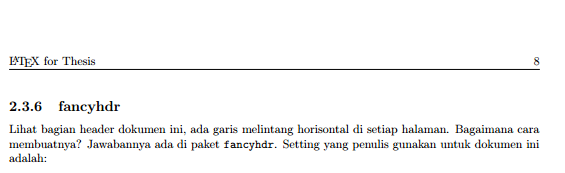
\includegraphics[width=10 cm]{img/6.png}
\end{figure}\\[0.5 cm]
Apabila Anda ingin menghilangkan garis horisontal pada bagian atas dan menggantinya dengan garis horisontal di bagian bawah, caranya:\\[0.5 cm]
\begin{tabular}{|p{13.5 cm}|}
\hline
 \textbackslash usepackage{fancyhdr}\\ 
 \textbackslash pagestyle{fancy} \\
   \textbackslash chead\{\} \\
   \textbackslash rhead\{\}  \\
   \textbackslash lhead\{\} \\
   \textbackslash rfoot\{\} \\
   \textbackslash lfoot\{\} \\
   \textbackslash cfoot\{\textbackslash thepage\}\\
  \textbackslash renewcommand\{\textbackslash headrulewidth\}\{0.0pt\}\\ 
 \textbackslash renewcommand\{\textbackslash footrulewidth\}\{0.4pt\}\\
\hline
\end{tabular}
\section{Daftar Pustaka}
Untuk menampilkan daftar pustaka atau bibliografi pada akhir sebuah dokumen LATEX digunakan format perintah seperti berikut ini :\\[0.5 cm]
\begin{tabular}{|p{13.5 cm}|}
\hline
 \textbackslash begin \{ thebibliography\}\{ 99 \} \\
 \textbackslash bibitem\{label untuk referensi\} \{ keterangan pustaka yang digunakan\}\\
.........\\
.........\\
 \textbackslash end\{thebibliography\}\\
\hline
\end{tabular}
\newpage
\begin{thebibliography}{99} 
\bibitem{hans01} 
{H.~Dulimarta, \emph{Pengenalan TEX dan LATEX}.\hskip 1em plus 0.5em minus 
0.4em\relax Home page : http://www.egr.msu.edu/dulimart, Januari 2001.} 
\bibitem{eitan94} 
{E.~M. Gurari, \emph{Writing With TeX}.\hskip 1em plus 0.5em minus 0.4em\relax 
MCGraw Hill, 1994.} 
\bibitem{lam94} 
{L.~Lamport, \emph{LATEX: A Document Preparation System}.\hskip 1em plus 0.5em 
minus 0.4em\relax Massachusetts: Addison-Wesley,Reading, 1994.} 
\bibitem{imim10} 
{I.~Z.pratama, \emph{form bekasi to medan with love}.\hskip 1em plus 0.5em minus 0.4em \relax bekasi : http//imranzulmi.blogspot.com, mei 2010.} 
\end{thebibliography} 
\newpage
Beberapa hal yang perlu diketahui dari perintah di atas antara lain :\\
\begin{itemize}
\item	Angka 99 memberitahu LATEX bahwa penomoran maksimal Daftar Pustaka adalah 99.
\item	Label untuk referensi diisikan keyword yang akan digunakan saat membuat rujukan ke pustaka yang bersangkutan.
\item	 Keterangan pustaka diisi informasi mengenai : penulis, judul pustaka, edisi, penerbit, kota penerbit, tahun penerbitan.
\end{itemize}
Cara untuk membuat rujukan ke salah satu pustaka yang sudah kita tuliskan dalam daftar pustaka adalah menggunakan perintah seperti ini :\\
\~{}\textbackslash cite\{label referensinya\}\\
Penggunaannya pada sebuah dokumen contohnya sebagai berikut :\\[0.5 cm]
\begin{tabular}{|p{13.5 cm}|}
\hline
\textbackslash begin\{thebibliography\}\{ 99\}\\
\textbackslash bibitem\{pustaka1\} \{ Peter Flynn : Begin \textbackslash LaTeX\textbackslash, Silmaril Consultants, (1999)\}\\
.........\\
.........\\
\textbackslash end\{thebibliography\}\\
\hline
\end{tabular}
\section{Notasi Matematika Dalam LATEX}
\subsection{Penulisan Notasi Matematika Dalam Paragraf}
Untuk menyisipkan notasi matematika dalam suatu kalimat/paragraf digunakan perintah berikut ini :\\[0.5 cm]
\begin{tabular}{|p{13.5 cm}|}
\hline
\textbackslash begin\{math\} ...... \textbackslash end\{math\} atau\\
\$ ...... \$\\

\hline
\end{tabular}\\[0.5 cm]
 Titik-titik merah tersebut di atas diisi dengan notasi matematis yang akan disisipkan.
\section{Paragraf Khusus Matematika}
Untuk menuliskan suatu notasi matematika yang cukup panjang, kita bisa memilih untuk menuliskannya dalam suatu paragraf baru. Perintah yang digunakan adalah sebagai berikut :\\[0.5 cm]
\begin{tabular}{|p{13.5 cm}|}
\hline
\textbackslash begin\{displaymath\}\\
......\\
\textbackslash end\{displaymath\}\\
\hline
\end{tabular}\\[0.5 cm]
Titik-titik merah tersebut di atas diisi dengan notasi matematis yang akan disisipkan.
\section{Font Dalam Matematika}
Ada beberapa perintah yang dapat digunakan untuk mengubah jenis font yang dipakai dalam notasi matematis, di antaranya adalah :\\
\begin{enumerate}
\item 	\textbackslash mathrm\{...\}
\item	\textbackslash mathsf\{...\}
\item	\textbackslash mathtt\{...\}
\item	\textbackslash mathit\{...\}
\item	\textbackslash mathbf\{...\}
\item	\textbackslash mathcal\{...\}
\end{enumerate}
\vspace{0.5 cm}
 Berikut adalah contoh hasil notasi matematis dengan masing-masing jenis font di atas :\\
\begin{enumerate}
\item Perintah \$\textbackslash mathrm\{x y x\}\$ akan menghasilkan : $\mathrm{xyz}$
\item  Perintah \$\textbackslash mathsf\{x y x\}\$ akan menghasilkan :   $\mathsf{xyz}$
\item  Perintah \$\textbackslash mathtt\{x y x\}\$ akan menghasilkan :    $\mathtt{xyz}$
\item  Perintah \$\textbackslash mathit\{x y x\}\$ akan menghasilkan :    $\mathit{xyz}$
\item  Perintah \$\textbackslash mathbf\{x y x\}\$ akan menghasilkan :   $\mathbf{xyz}$
\item  Perintah \$\textbackslash mathcal\{X Y Z\}\$ akan menghasilkan:  $\mathcal{XYZ}$
\end{enumerate}
 Untuk menuliskan font matematika dalam bentuk superscripts dan subscripts digunakan aturan berikut ini :
\begin{itemize}
\item Superscripts , cara penulisannya adalah dengan perintah \textbackslash sp\{...\} atau dengan tanda\^{}.
\item  Subscript , cara penulisannya adalah dengan perintah \textbackslash sb\{...\} atau dengan tanda .

\end{itemize}
Contoh pemakaiannya sebagai berikut :\\[0.5 cm]
\begin{tabular}{|p{13.5 cm}|}
\hline
\textbackslash begin\{displaymath\}\\
    y = x\textbackslash sb\{1\}\textbackslash sp\{2\} + x\textbackslash sb\{2\}\textbackslash sp\{2\}\\
\textbackslash end\{displaymath\}\\
\hline
\end{tabular}\\[0.5 cm]
Perintah di atas akan menghasilkan keluaran seperti berikut :\\[0.5 cm]
\begin{displaymath}
    y = x\sb{1}\sp{2} + x\sb{2}\sp{2}
\end{displaymath}\\[0.5 cm]
Contoh lainnya :\\[0.5 cm]
\begin{tabular}{|p{13.5 cm}|}
\hline
\textbackslash begin\{displaymath\}\\
    y =f(x)=e\^{}\{x 1\}\\
\textbackslash end\{displaymath\}\\
\hline
\end{tabular}\\[0.5 cm]
Perintah di atas akan menghasilkan keluaran seperti berikut :\\[0.5 cm]
\begin{displaymath}
f(x)=e^{x1}	
\end{displaymath}\\[0.5 cm]
Notasi matematika sering menggunakan huruf-huruf Yunani. Tabel 5.1 berikut ini memuat daftar huruf kecil Yunani dan cara penulisannya dalam LATEX :\\
\begin{figure}[h!]
\centering
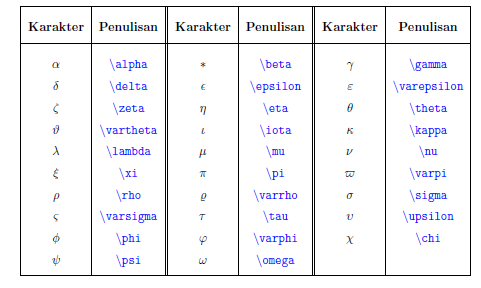
\includegraphics[width=10 cm]{img/10.png}
\end{figure}
\begin{raggedleft}Tabel 5.2 berikut ini memuat huruf kapital Yunani dan cara penulisannya dalam  LATEX\end{raggedleft}\\[0.5 cm]
\begin{figure}[h!]
\centering
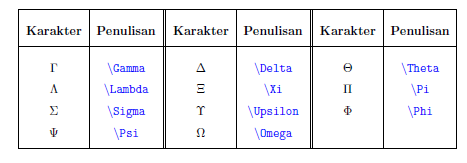
\includegraphics[width=10 cm]{img/11.png}
\end{figure}
\section{Tanda Kurung Dalam Matematika}
Penulisan tanda kurung dalam notasi matematis tidak bisa2 menggunakan tanda kurung biasa. Cara penulisan yang akan mengeluarkan notasi matematika yang baik adalah sebagai berikut :\\[0.5 cm]
\begin{tabular}{lll}
\textbackslash right delimiter& :& untuk menghasilkan tanda kurung sebelah kanan\\
\textbackslash left delimiter& : &untuk menghasilkan tanda kurung sebelah kiri\\
\end{tabular}\\[0.5 cm]
Delimiter sendiri adalah tanda kurung biasa yang penulisannya tentunya sesuai standar perintah LATEX . Beberapa delimiter yang biasa digunakan dalam notasi matematika ditunjukkan dalam Tabel 5.3 :\\[0.5 cm]
\begin{figure}[h!]
\centering
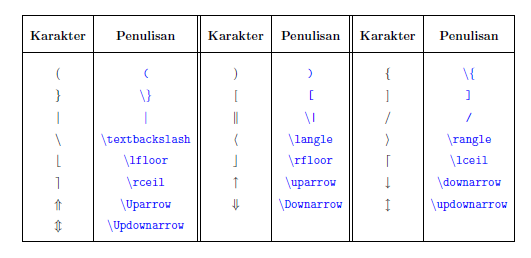
\includegraphics[width=10 cm]{img/12.png}
\end{figure}\\[0.5 cm]
\section{Penulisan Akar}
Format perintah untuk menghasilkan akar matematik adalah sebagai berikut:\\[0.5 cm]
\begin{tabular}{|p{13.5 cm}|}
\hline
\textbackslash sqrt[pangkat]\{bilangan yang diakar\}\\
\hline
\end{tabular}\\[0.5 cm]
  Contoh pemakaiannya adalah sebagai berikut :\\[0.5 cm]
\begin{tabular}{|p{13.5 cm}|}
\hline
\textbackslash begin\{displaymath\}\\
   \textbackslash sqrt[2]\{a+b\}\\
\textbackslash end\{displaymath\}\\
\hline
\end{tabular}\\[0.5 cm]
 Perintah di atas akan menghasilkan notasi seperti berikut :\\[0.5 cm]
\begin{displaymath}
\sqrt[2]{a+b}
\end{displaymath}
\section{Penulisan Pecahan}
Format perintah untuk menghasilkan notasi pecahan adalah sebagai berikut :\\[0.5 cm]
\begin{tabular}{|p{13.5 cm}|}
\hline
\textbackslash frac\{numerator\}\{denominator\}\\
\hline
\end{tabular}\\[0.5 cm]
Contoh pemakaiannya adalah sebagai berikut :\\[0.5 cm]
\begin{tabular}{|p{13.5 cm}|}
\hline
\textbackslash begin\{displaymath\}\\
   \textbackslash frac\{12x\}\{x+1\}\\
\textbackslash end\{displaymath\}\\
\hline
\end{tabular}\\[0.5 cm]
Perintah di atas akan menghasilkan notasi seperti berikut :\\[0.5 cm]
\begin{displaymath}
\frac{12x}{x+1}
\end{displaymath}
\section{Penulisan Array \& Matriks}
Sebuah array/matriks dituliskan dalam environment tabular sama seperti cara pembuatan
tabel. Perintah untuk menghasilkan sebuah array atau matriks adalah seperti berikut :\\[0.5 cm]
\begin{tabular}{|p{13.5 cm}|}
\hline
\textbackslash begin\{displaymath\}\\
   \textbackslash left (\\
\textbackslash begin\{array\}\{rrr\}\\
0 \& 45 \& 23 \\
34\& -93 \& 68 \textbackslash end\{array\}\\
\textbackslash right )\\

\textbackslash end\{displaymath\}\\
\hline
\end{tabular}\\[0.5 cm]
Contoh perintah di atas akan menghasilkan matriks seperti berikut ini :\\[0.5 cm]
\begin{displaymath}
\left (
\begin{array}{rrr}
0 & 45 & 23 \\
34& -93 & 68 \end{array}
\right )
\end{displaymath}\\[0.5 cm]
Beberapa hal yang perlu diketahui dari format perintah tersebut di atas :
\begin{itemize}
\item	Sama seperti cara penulisan tabel, huruf r di bagian belakang \textbackslash begin\\\{array\}\{rrr\} fungsinya adalah menentukan posisi dari masing-masing komponen matriks tersebut. Dalam hal ini masing-masing komponen matriks dibuat menjadi rata kanan.
\item	Tanda kurung yang digunakan adalah berupa tanda kurung kurawal. Bagian kurung buka dan kurung tutup didefinisikan masing-masing.
\end{itemize}
\section{Penulisan  Vektors}
Penulisan vektor dalam LATEX menggunakan perintah seperti berikut ini :\\[0.5 cm]
\begin{tabular}{|p{13.5 cm}|}
\hline
\textbackslash begin\{displaymath\}\\
\textbackslash vec\{variabel\}

\textbackslash end\{displaymath\}\\
\hline
\end{tabular}\\[0.5 cm]
Misalnya :\\[0.5 cm]
\begin{tabular}{|p{13.5 cm}|}
\hline
\textbackslash begin\{displaymath\}\\
\textbackslash vec\{x\}

\textbackslash end\{displaymath\}\\
\hline
\end{tabular}\\[0.5 cm]
akan menghasilkan vector seperti :\\[0.5 cm]
\begin{displaymath}
\vec{x}
\end{displaymath}
\section{Penulisan Fungsi Matematika}
Ada cukup banyak fungsi matematika yang memiliki perintah khusus untuk menuliskannya
dalam dokumen LATEX seperti misalnya sinus, cosinus, dll. Berikut adalah  tabel yang
menampilkan beberapa fungsi tersebut :\\[0.5 cm]
\begin{figure}[h!]
\centering
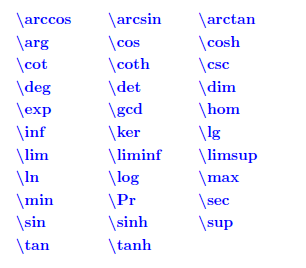
\includegraphics[width=7 cm]{img/13.png}
\end{figure}
\newpage
\section{Simbol-Simbol Matematika}
\begin{raggedleft}Untuk dapat menggunakan berbagai simbol matematika, kita harus mendeklarasikan penggunaan paket amsmath pada bagian preamble. Berikut menunjukkan simbol-simbol matematika serta perintah penulisannya dalam LATEX .\end{raggedleft}\\[0.5 cm]
\begin{figure}[h!]
\centering
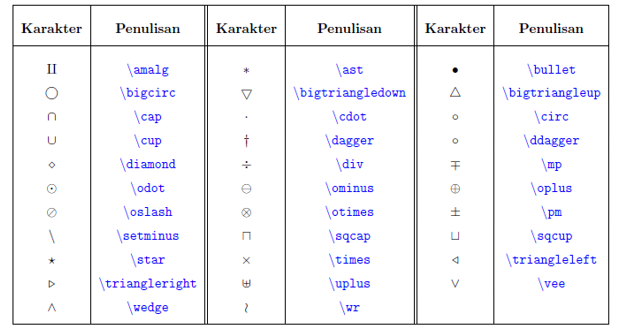
\includegraphics[width=10 cm]{img/14.png}
\end{figure}

\begin{figure}[h!]
\centering
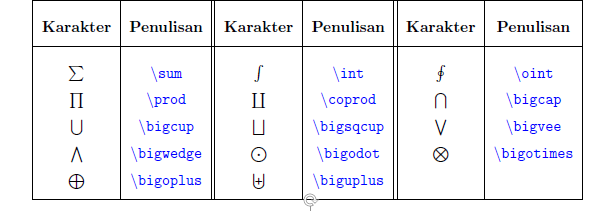
\includegraphics[width=10 cm]{img/15.png}
\end{figure}

\begin{figure}[h!]
\centering
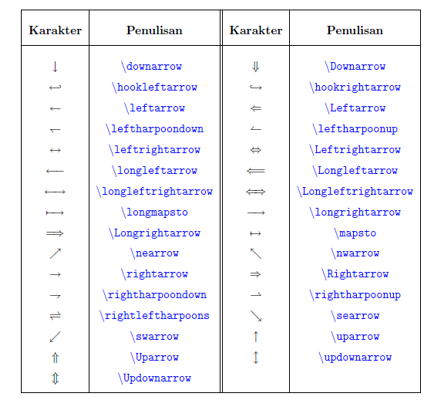
\includegraphics[width=10 cm]{img/16.png}
\end{figure}

\begin{figure}[h!]
\centering
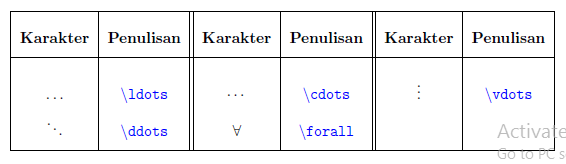
\includegraphics[width=10 cm]{img/17.png}
\end{figure}
\newpage
\section{Membuat halaman landscape dan portrait}
Dalam latex, dapat membuat dan meletakkan dokumen dengan landscape maupun  portrait sebagai contoh:\\[0.5 cm]
\begin{tabular}{|p{13.5 cm}|}
\hline
\textbackslash documentclass[12pt,a4paper]\{report\}\\
\textbackslash usepackage\{lscape\}\\
\textbackslash begin\{document\}\\
\textbackslash  pagenumbering\{arabic\}\\
\textbackslash chapter\{Title 1\}\\
\textbackslash  begin\{landscape\}\\
\textbackslash centering\\
Text here.\\
\textbackslash end\{landscape\}\\
\textbackslash  chapter\{Title 2\}\\
\textbackslash  end\{document\}\\
\hline
\end{tabular}\\[0.5 cm]
hasil output-nya:\\
\begin{enumerate}
\item halaman pertama
\begin{figure}[h!]
\centering
\fbox{
\includegraphics[width=10 cm]{img/28.png}}
\end{figure}
\item halaman kedua
\begin{figure}[h!]
\centering
\fbox{
\includegraphics[width=10 cm]{img/29.png}}
\end{figure}
\newpage
\item halaman ketiga
\begin{figure}[h!]
\centering
\fbox{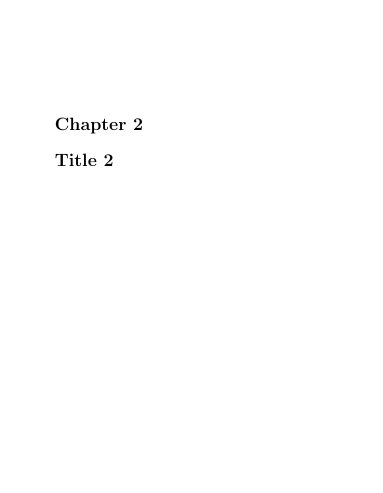
\includegraphics[width=10 cm]{img/30.png}}
\end{figure}
\end{enumerate}
\section{memberikan warna dalam tabel}
Dalam latex, kita dapat memberikan waarna pada setiap baris maupun kolom dalam tabel sebagai contoh sebagai berikut:\\[0.5cm]
\begin{enumerate}
\newpage
\item perwarnaan pada baris tabel\\
\begin{tabular}{|p{12.5 cm}|}
\hline
\textbackslash documentclass[11pt,a4paper]\{article\}\\
\textbackslash usepackage[T1]\{fontenc\}\\
\textbackslash usepackage[latin1]\{inputenc\}\\
\textbackslash usepackage[table]\{xcolor\}\\    % loads also »colortbl«

\textbackslash begin\{document\}\\
  \textbackslash rowcolors\{2\}\{gray!25\}\{white\}\\
  \textbackslash begin\{tabular\}\{cc\}\\
    \textbackslash rowcolor\{gray!50\}\\
    Table head \& Table head  \textbackslash \textbackslash \\
    Some values \& Some values\textbackslash \textbackslash  \\
    Some values \& Some values \textbackslash \textbackslash \\
    Some values \& Some values \textbackslash \textbackslash  \\
    Some values \& Some values\\
  \textbackslash  end\{tabular\}\\
\textbackslash end\{document\}\\
\hline
\end{tabular}\\[0.5 cm]
 hasil outputnya:\\
\begin{figure}[h!]
\centering
\fbox{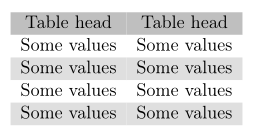
\includegraphics[width=10 cm]{img/31.png}}
\end{figure}
\newpage
\item perwarnaan pada kolom tabel\\
\begin{tabular}{|p{12.5 cm}|}
\hline
 \textbackslash newcolumntype\{g\}\{\textgreater \{ \textbackslash columncolor\{red\}\}c\}\\
 \textbackslash begin\{table\}[ht]\\
 \textbackslash centering\\
 \textbackslash begin\{tabular\}\{c \textbar g \textbar c \textbar g\textbar c \textbar g\textbar c\textbar g\}\\
 \textbackslash hline\\
\&col1 \&col2 \&col3 \&col4 \& col5 \&col6 \&col7\textbackslash\textbackslash\\
 \textbackslash hline \\
row1\& 1 \&2 \& 3  \& 4 \& 5 \& 6 \&7 \textbackslash \textbackslash\\
row2\& 2 \& 3 \& 5 \& 6 \& 7 \& 1 \& 1 \textbackslash\textbackslash\\
row3\& 3 \& 4 \& 6 \& 7 \& 1 \& 2 \& 2 \textbackslash\textbackslash \\
row4\& 4 \& 5 \& 7\& 1 \& 2 \& 3 \& 3  \textbackslash\textbackslash\\
row5\& 5 \& 6 \& 1\& 2 \& 3 \& 4 \& 4  \textbackslash\textbackslash\\
row6\& 6 \& 7 \& 2 \& 3 \& 4 \& 5 \& 5  \textbackslash\textbackslash\\
\textbackslash hline\\
  \textbackslash  end\{tabular\}\\
  \textbackslash  end\{table\}\\
\hline
\end{tabular}\\[0.5 cm]
 hasil outputnya:\\
\newcolumntype{g}{>{\columncolor{yellow}}c}
\begin{tabular}{c|g|c|g|c|g|c|g}
\hline
       &col1 &col2 &col3 &col4 & col5 &col6 &col7\\
\hline
row1& 1 &2 & 3  & 4 & 5 & 6 &7\\
row2& 2 & 3 & 5 & 6 & 7 & 1 & 1 \\
row3& 3 & 4 & 6 & 7 & 1 & 2 & 2 \\
row4& 4 & 5 & 7& 1 & 2 & 3 & 3 \\
row5& 5 & 6 & 1 & 2 & 3 & 4 & 4 \\
row6& 6 & 7 & 2 & 3 & 4 & 5 & 5 \\
\hline
\end{tabular}
\end{enumerate}
\section{mengubah {\itshape font size} dalam tabel}
Dalam tabel kita dapat mengubah {\itshape font size} yang sesuai yang kita inginkan. Berikut contoh {\itshape source code} yang digunakan: \\[0.5 cm]
\begin{tabular}{|p{13.5 cm}|}
\hline
    \textbackslash fontsize\{10pt\}\{20pt\}\\
      \textbackslash selectfont\\

    ...table...\\

      \textbackslash fontsize\{11pt\}\{21pt\}\\
      \textbackslash selectfont\\
\hline
\end{tabular}
\section{ mengatur {\itshape margin}}
Dalam membuat dokumen, kita dapat mengatur {\itshape margin} berikut contoh kode yang digunakan:\\[0.5 cm]
\begin{tabular}{|p{13.5 cm}|}
\hline
\textbackslash usepackage[left=2cm, right=5cm, top=2cm]\{geometry\}\\
\hline
\end{tabular}
\section{Menambahkan nama pada daftar isi , daftar tabel dan daftar gambar}
\begin{enumerate}
\item Memberikan nama BAB  di tiap {\itshape chapter} dalam daftar isi.\\
\begin{tabular}{|p{12.5 cm}|}
\hline
\textbackslash renewcommand\{\textbackslash cftchappresnum\}\{BAB  \} \\
\textbackslash AtBeginDocument\{\textbackslash addtolength\textbackslash cftchapnumwidth\{\textbackslash widthof\{\textbackslash bfseries Chapter\}\}\} \\
\hline
\end{tabular}
\item  Memberikan nama Tabel di  dalam daftar tabel.\\
\begin{tabular}{|p{12.5 cm}|}
\hline
\{ \\
\textbackslash let\textbackslash oldnumberline\textbackslash numberline \\
\textbackslash renewcommand\{\textbackslash numberline\}\{\textbackslash tablename~~\textbackslash oldnumberline\} \\
\textbackslash listoftables\\
\} \\
\hline
\end{tabular}
\item  Memberikan nama Gambar di dalam daftar gambar.\\
\begin{tabular}{|p{12.5 cm}|}
\hline
\{ \\
\textbackslash let\textbackslash oldnumberline\textbackslash numberline\\
\textbackslash renewcommand\{\textbackslash numberline\}\{\textbackslash figurename~~\textbackslash oldnumberline\} \\
\textbackslash listoffigures\\
\} \\
\hline
\end{tabular}
\end{enumerate}
	
	\setcounter{page}{1}
	\chapter{PENDAHULUAN}
\section{Latar Belakang}
Mea tale aliquam minimum te. Eu mel putant virtute, essent inermis nominavi mea no. Laoreet indoctum sea te. Te scripta fabulas duo, pro doming recusabo voluptaria at. Cu sed numquam inciderint, ei minim altera disputando cum, te nec graeco maiorum convenire.\\
Cu mel putent rationibus dissentiet. Per vidisse scaevola oportere ei, qui solet molestie eu. Hinc diceret nominati per at, nec dico denique laboramus et. Legere regione his at, aeque decore in mei.Aliquam tincidunt a nulla ac posuere. Maecenas sapien mi, feugiat sit amet tellus at, dictum varius ante. Cras rutrum facilisis felis at hendrerit. Nullam eleifend sed lorem a iaculis. Donec ut odio at nisl molestie euismod quis et purus. Curabitur eu ex turpis. Etiam maximus metus non iaculis placerat. Sed in risus sodales, posuere elit in, eleifend tellus. Mauris at consectetur arcu. Integer fringilla eros mi, vel volutpat enim commodo ac.\\

Suspendisse ac porta diam, ut viverra ante. Aliquam mattis tincidunt diam in molestie. Sed auctor fermentum turpis, sed varius ante. Nulla rutrum, enim et efficitur dignissim, urna diam consequat purus, sit amet elementum nibh mauris ut tellus. Quisque interdum leo ligula, a volutpat mauris viverra ut. Fusce ac felis finibus, convallis ligula a, aliquam nunc. Quisque faucibus ligula et ornare finibus. Morbi maximus dolor vitae dolor tristique, eu sagittis metus auctor. Pellentesque quam lacus, ornare ut est ut, egestas auctor leo. Duis eros neque, mollis quis elit id, cursus egestas neque. Pellentesque ac sapien vitae nulla varius rhoncus. Orci varius natoque penatibus et magnis dis parturient montes, nascetur ridiculus mus. Etiam pharetra nisl et massa facilisis aliquet. Nulla sit amet quam enim. Nunc dictum pellentesque orci, at sollicitudin erat condimentum eu. Nullam mi dolor, vestibulum at lacinia quis, feugiat faucibus felis.\\

\section{Rumusan Masalah}
Etiam pharetra nisl et massa facilisis aliquet.
\begin{enumerate}[nolistsep,leftmargin=0.5cm]
  \item Suspendisse ac porta diam?
  \item Suspendisse ac porta diam?\\
\end{enumerate}

\section{Tujuan Penelitian}
Etiam pharetra nisl et massa facilisis aliquet.
\begin{enumerate}[nolistsep,leftmargin=0.5cm]
  \item Suspendisse ac porta diam.
  \item Suspendisse ac porta diam.\\
\end{enumerate}

\section{Batasan Masalah}
Suspendisse ac porta diam, ut viverra ante. Aliquam mattis tincidunt diam in molestie. Sed auctor fermentum turpis, sed varius ante. Nulla rutrum, enim et efficitur dignissim, urna diam consequat purus, sit amet elementum nibh mauris ut tellus. Quisque interdum leo ligula, a volutpat mauris viverra ut. Fusce ac felis finibus, convallis ligula a, aliquam nunc. Quisque faucibus ligula et ornare finibus.
\begin{enumerate}[nolistsep,leftmargin=0.5cm]
  \item Suspendisse ac porta diam.
  \item Suspendisse ac porta diam.
  \item Feugiat faucibus felis.\\
\end{enumerate}

\section{Konstribusi Penelitian}
Suspendisse ac porta diam, ut viverra ante. Aliquam mattis tincidunt diam in molestie. Sed auctor fermentum turpis, sed varius ante. Nulla rutrum, enim et efficitur dignissim, urna diam consequat purus, sit amet elementum nibh mauris ut tellus. Quisque interdum leo ligula, a volutpat mauris viverra ut. Fusce ac felis finibus, convallis ligula a, aliquam nunc. Quisque faucibus ligula et ornare finibus. Morbi maximus dolor vitae dolor tristique, eu sagittis metus auctor. Pellentesque quam lacus, ornare ut est ut, egestas auctor leo. Duis eros neque, mollis quis elit id, cursus egestas neque. Pellentesque ac sapien vitae nulla varius rhoncus. Orci varius natoque penatibus et magnis dis parturient montes, nascetur ridiculus mus. Etiam pharetra nisl et massa facilisis aliquet. Nulla sit amet quam enim. Nunc dictum pellentesque orci, at sollicitudin erat condimentum eu. Nullam mi dolor, vestibulum at lacinia quis, feugiat faucibus felis.\\

\section{Metodologi Penelitian}
Suspendisse ac porta diam, ut viverra ante. Aliquam mattis tincidunt diam in molestie. Sed auctor fermentum turpis, sed varius ante. Nulla rutrum, enim et efficitur dignissim, urna diam consequat purus, sit amet elementum nibh mauris ut tellus. Quisque interdum leo ligula, a volutpat mauris viverra ut. Fusce ac felis finibus, convallis ligula a, aliquam nunc. Quisque faucibus ligula et ornare finibus. Morbi maximus dolor vitae dolor tristique, eu sagittis metus auctor. Pellentesque quam lacus, ornare ut est ut, egestas auctor leo. Duis eros neque, mollis quis elit id, cursus egestas neque. Pellentesque ac sapien vitae nulla varius rhoncus. Orci varius natoque penatibus et magnis dis parturient montes, nascetur ridiculus mus. Etiam pharetra nisl et massa facilisis aliquet. Nulla sit amet quam enim. Nunc dictum pellentesque orci, at sollicitudin erat condimentum eu. Nullam mi dolor, vestibulum at lacinia quis, feugiat faucibus felis.\\

\section{Sistematika Pembahasan}
Bab 1: cursus egestas neque
Suspendisse ac porta diam, ut viverra ante. Aliquam mattis tincidunt diam in molestie. Sed auctor fermentum turpis, sed varius ante. Nulla rutrum, enim et efficitur dignissim, urna diam consequat purus, sit amet elementum nibh mauris ut tellus. Quisque interdum leo ligula, a volutpat mauris viverra ut. Fusce ac felis finibus, convallis ligula a, aliquam nunc.\\

Bab 2: cursus egestas neque
Suspendisse ac porta diam, ut viverra ante. Aliquam mattis tincidunt diam in molestie. Sed auctor fermentum turpis, sed varius ante. Nulla rutrum, enim et efficitur dignissim, urna diam consequat purus, sit amet elementum nibh mauris ut tellus. Quisque interdum leo ligula, a volutpat mauris viverra ut. Fusce ac felis finibus, convallis ligula a, aliquam nunc.\\

Bab 3: cursus egestas neque
Suspendisse ac porta diam, ut viverra ante. Aliquam mattis tincidunt diam in molestie. Sed auctor fermentum turpis, sed varius ante. Nulla rutrum, enim et efficitur dignissim, urna diam consequat purus, sit amet elementum nibh mauris ut tellus. Quisque interdum leo ligula, a volutpat mauris viverra ut. Fusce ac felis finibus, convallis ligula a, aliquam nunc.\\

Bab 4: cursus egestas neque
Suspendisse ac porta diam, ut viverra ante. Aliquam mattis tincidunt diam in molestie. Sed auctor fermentum turpis, sed varius ante. Nulla rutrum, enim et efficitur dignissim, urna diam consequat purus, sit amet elementum nibh mauris ut tellus. Quisque interdum leo ligula, a volutpat mauris viverra ut. Fusce ac felis finibus, convallis ligula a, aliquam nunc.\\

Bab 5: cursus egestas neque
Suspendisse ac porta diam, ut viverra ante. Aliquam mattis tincidunt diam in molestie. Sed auctor fermentum turpis, sed varius ante. Nulla rutrum, enim et efficitur dignissim, urna diam consequat purus, sit amet elementum nibh mauris ut tellus. Quisque interdum leo ligula, a volutpat mauris viverra ut. Fusce ac felis finibus, convallis ligula a, aliquam nunc.\\
	
	\setcounter{page}{1}
	%-----------------------------------------------------------------------------%
\chapter{LANDASAN TEORI}
%-----------------------------------------------------------------------------%
\vspace{4.5pt}

\section{Tinjauan Pustaka}

\subsection{Judul Bagian}
Mea tale aliquam minimum te. Eu mel putant virtute, essent inermis nominavi mea no. Laoreet indoctum sea te. Te scripta fabulas duo, pro doming recusabo voluptaria at. Cu sed numquam inciderint, ei minim altera disputando cum, te nec graeco maiorum convenire.\\
Cu mel putent rationibus dissentiet. Per vidisse scaevola oportere ei, qui solet molestie eu. Hinc diceret nominati per at, nec dico denique laboramus et. Legere regione his at, aeque decore in mei \cite{1}. \textit{Cite} merupakan href.\\

\subsubsection{Judul\_Sub\_Bagian\_1}
Mea tale aliquam minimum te. Eu mel putant virtute, essent inermis nominavi mea no. Laoreet indoctum sea te. Te scripta fabulas duo, pro doming recusabo voluptaria at. Cu sed numquam inciderint, ei minim altera disputando cum, te nec graeco maiorum convenire.\\
Cu mel putent rationibus dissentiet. Per vidisse scaevola oportere ei, qui solet molestie eu. Hinc diceret nominati per at, nec dico denique laboramus et. Legere regione his at, aeque decore in mei \cite{sosmed}. \textit{Cite} merupakan href.\\\\

\subsubsection{Judul\_Sub\_Bagian\_2}
Mea tale aliquam minimum te. Eu mel putant virtute, essent inermis nominavi mea no. Laoreet indoctum sea te. Te scripta fabulas duo, pro doming recusabo voluptaria at. Cu sed numquam inciderint, ei minim altera disputando cum, te nec graeco maiorum convenire.\\
Cu mel putent rationibus dissentiet. Per vidisse scaevola oportere ei, qui solet molestie eu. Hinc diceret nominati per at, nec dico denique laboramus et. Legere regione his at, aeque decore in mei \cite{sosmed}. \textit{Cite} merupakan href.\\\\

Persamaan \ref{eq:persamaan 1} merupakan href. Persamaan \ref{eq:qwer} merupakan href. 

\begin{flalign}
	\hspace{1.5cm}
	&x_{y+1}[z] = (a_{b}[-c] * d_{e}[f]) \downarrow 2& 
	\label{eq:persamaan 1} \\
	&x_{y+1}[z] = (a_{b}[-c] * d_{e}[f]) \uparrow 2& 
	\label{eq:qwer}
\end{flalign}
\begin{table}[H]
	\begin{adjustbox}{width=1\textwidth}
		\begin{tabular}{lp{13.55cm}l}
			\hline \\
			Di mana&:\\
			$x_{y+1}[z]]$ &:aasdfghjkl \\
			$a_{b}[-c]$ &: qwertyuiop \\
			$d_{e}[f]$ &: zxcvbnm\\
			$\downarrow 2$ &: Operasi \textit{downsample} \\
			$\uparrow 2$ &: Operasi \textit{upsample} \\
			\hline
		\end{tabular}
	\end{adjustbox}
\end{table}

\begin{table}
	\small
	\begin{adjustbox}{width=1\textwidth}
		\begin{tabular}{|p{13.55cm}|}
			\hline
			
			\begin{equation}
			\label{eq: fgh}
			vidisse = rationibus - graeco
			\end{equation}
			
			\begin{equation}
			\label{eq: asd}
			decore = \left\{
			\begin{array}{rcl}
				Legere & \mbox{mei} & decore > 0 \\
				NeuLegeretral & \mbox{mei} & decore = 0 \\
				aeque & \mbox{mei} & decore < 0 
			\end{array}\right.
			\end{equation}\\
			
			\hline
		\end{tabular}
	\end{adjustbox}
\end{table}
\indent Keterangan: 

\indent \textit{Legere} = llualsdmf. \\
\indent \textit{decore} = oievjad. \\
\indent \textit{NeuLegeretral} = Bias. \\
\indent \textit{aeque} = uwuiopd.\\

Mea tale aliquam minimum te. Eu mel putant virtute, essent inermis nominavi mea no. Laoreet indoctum sea te:

\begin{algorithm} 
  \begin{algorithmic}[1]
    \REQUIRE $n \geq 0$
    \ENSURE $y = x^n$
    \STATE $y \gets 1$
    \STATE $X \gets x$
    \STATE $N \gets n$
    \WHILE{$N \neq 0$}
    \IF{$N$ is even}
        \STATE $X \gets X \times X$
        \STATE $N \gets \frac{N}{2}$  \COMMENT{This is a comment}
    \ELSIF{$N$ is odd}
        \STATE $y \gets y \times X$
        \STATE $N \gets N - 1$
    \ENDIF
    \ENDWHILE
  \end{algorithmic} 
  \caption{A test algorithm}
  \label{alg:algorithm1}
\end{algorithm}

Algorithm~\ref{alg:algorithm1} states blah blah blah and algorithm~\ref{alg:algorithm2} states blah blah blah. \\

\begin{algorithm} 
  \begin{algorithmic}[1]
    \STATE $i \gets 10$
    \IF{$i\geq 5$} 
        \STATE $i \gets i-1$
    \ELSE
        \IF{$i\leq 3$}
            \STATE $i \gets i+2$
        \ENDIF
    \ENDIF 
    \RETURN{}
  \end{algorithmic} 
  \caption{Another test algorithm}
  \label{alg:algorithm2}
\end{algorithm}

\subsection{Judul Bagian 2}
Mea tale aliquam minimum te. Eu mel putant virtute, essent inermis nominavi mea no. Laoreet indoctum sea te. Te scripta fabulas duo, pro doming recusabo voluptaria at. Cu sed numquam inciderint, ei minim altera disputando cum, te nec graeco maiorum convenire. Cu mel putent rationibus dissentiet. Per vidisse scaevola oportere ei, qui solet molestie eu. Hinc diceret nominati per at, nec dico denique laboramus et. Legere regione his at, aeque decore in mei.\\

Mea tale aliquam minimum te. Eu mel putant virtute, essent inermis nominavi mea no. Laoreet indoctum sea te. Te scripta fabulas duo, pro doming recusabo voluptaria at. Cu sed numquam inciderint, ei minim altera disputando cum, te nec graeco maiorum convenire.Cu mel putent rationibus dissentiet. Per vidisse scaevola oportere ei, qui solet molestie eu. Hinc diceret nominati per at, nec dico denique laboramus et. Legere regione his at, aeque decore in. Mea tale aliquam minimum te. Eu mel putant virtute, essent inermis nominavi mea no. Laoreet indoctum sea te. Te scripta fabulas duo, pro doming recusabo voluptaria at. Cu sed numquam inciderint, ei minim altera disputando cum, te nec graeco maiorum convenire.\\

\subsection{Pustaka Pendukung}
Suspendisse ac porta diam, ut viverra ante. Aliquam mattis tincidunt diam in molestie. Sed auctor fermentum turpis, sed varius ante. Nulla rutrum, enim et efficitur dignissim, urna diam consequat purus, sit amet elementum nibh mauris ut tellus. Quisque interdum leo ligula, a volutpat mauris viverra ut. Fusce ac felis finibus, convallis ligula a, aliquam nunc. Quisque faucibus ligula et ornare finibus. Morbi maximus dolor vitae dolor tristique, eu sagittis metus auctor. Pellentesque quam lacus, ornare ut est ut, egestas auctor leo. Duis eros neque, mollis quis elit id, cursus egestas neque.\\
\begin{small}
	\begin{longtable}[c]{|p{0.4cm}|p{3cm}|p{2.8cm}|p{1.8cm}|p{3.8cm}|}
		\caption{Daftar \textit{method} yang digunakan dari pustaka\textit{ Library\_1}}
		\label{library:Library1}\\
		\hline
		\centering \textbf{No.} &
		\centering \textbf{\textit{Method}} &
		\centering \textbf{Masukan} &
		\centering \textbf{Luaran} &
		\centering \textbf{Keterangan} \tabularnewline \hline
		\multirow{2}{*}{1.} & Flask & \_\_name\_\_ : string & - & \textit{Constructor} dari objek Flask dimana objek merepresentasikan aplikasi \textit{web} yang digunakan. Pada penelitian ini objek diinisialisasi dengan mendefinisikan direktori \textit{static} yang digunakan untuk menyimpan \textit{file} secara \textit{local}.\\
        \cline{3-3}
        & & static\_url\_path : string\newline static\_folder : string & & \\ \hline
		2. & render\_template & template\_name : string & HTML & Menampilkan halaman yang didefinisikan. \\ \hline
		3. & request & - & - & Objek yang secara otomatis diinisialisasi untuk merepresentasikan \textit{request} yang dikitim dari UI. \\ \hline
		4. & route & name : string \newline method : string[] & - & Mendefinisikan \textit{routing} yang akan digunakan. \\ \hline
		5. & send\_from\_directory & directory : string\newline filename : string & File & Mengambil \textit{file} dari direktori \textit{static}. \\ \hline
		6. & run & - & - & Menjalankan objek Flask yang telah diinisialisasi. \\ \hline
		
	\end{longtable}
\end{small}

\section{Tinjauan Studi}
\par Pada Tabel \ref{tbl:StateoftheArt} diberikan penjelasan mengenai studi terkait dalam penelitian:

\begingroup
\setlength{\LTleft}{-20cm plus -1fill}
\setlength{\LTright}{\LTleft}
\begin{small}
	\begin{longtable}{|p{0.5cm}|p{2.7cm}|p{3.2cm}|p{3.1cm}|p{2.5cm}|}
		\caption{Tinjauan Studi}\\
		\hline
		\textbf{No} & \textbf{Peneliti} & \textbf{Judul} & \textbf{Rumusan Masalah} & \textbf{Hasil}\\
		\endfirsthead
		
		\hline
		1 & Suspendisse ac porta diam, ut viverra ante. & Aliquam mattis tincidunt diam in molestie. Sed auctor fermentum turpis, sed varius ante. Nulla rutrum, enim et efficitur dignissim, urna diam consequat purus, sit amet elementum nibh mauris ut tellus. & Quisque interdum leo ligula, a volutpat mauris viverra ut. Fusce ac felis finibus, convallis ligula a, aliquam nunc. & Quisque faucibus ligula et ornare finibus. Morbi maximus dolor vitae dolor tristique, eu sagittis metus auctor. Pellentesque quam lacus, ornare ut est ut, egestas auctor leo. Duis eros neque, mollis quis elit id, cursus egestas neque.\\
		
		\hline
		2 & Suspendisse ac porta diam, ut viverra ante. & Aliquam mattis tincidunt diam in molestie. Sed auctor fermentum turpis, sed varius ante. Nulla rutrum, enim et efficitur dignissim, urna diam consequat purus, sit amet elementum nibh mauris ut tellus. & Quisque interdum leo ligula, a volutpat mauris viverra ut. Fusce ac felis finibus, convallis ligula a, aliquam nunc. & Quisque faucibus ligula et ornare finibus. Morbi maximus dolor vitae dolor tristique, eu sagittis metus auctor. Pellentesque quam lacus, ornare ut est ut, egestas auctor leo. Duis eros neque, mollis quis elit id, cursus egestas neque.\\
		
		\hline
		3 & Suspendisse ac porta diam, ut viverra ante. & Aliquam mattis tincidunt diam in molestie. Sed auctor fermentum turpis, sed varius ante. Nulla rutrum, enim et efficitur dignissim, urna diam consequat purus, sit amet elementum nibh mauris ut tellus. & Quisque interdum leo ligula, a volutpat mauris viverra ut. Fusce ac felis finibus, convallis ligula a, aliquam nunc. & Quisque faucibus ligula et ornare finibus. Morbi maximus dolor vitae dolor tristique, eu sagittis metus auctor. Pellentesque quam lacus, ornare ut est ut, egestas auctor leo. Duis eros neque, mollis quis elit id, cursus egestas neque.
		\label{tbl:StateoftheArt}\\
		\hline
	\end{longtable}
\end{small}
\endgroup
Mea tale aliquam minimum te. Eu mel putant virtute, essent inermis nominavi mea no. Laoreet indoctum sea te. Te scripta fabulas duo, pro doming recusabo voluptaria at. Cu sed numquam inciderint, ei minim altera disputando cum, te nec graeco maiorum convenire. Cu mel putent rationibus dissentiet. Per vidisse scaevola oportere ei, qui solet molestie eu. Hinc diceret nominati per at, nec dico denique laboramus et. Legere regione his at, aeque decore in mei.\\

Mea tale aliquam minimum te. Eu mel putant virtute, essent inermis nominavi mea no. Laoreet indoctum sea te. Te scripta fabulas duo, pro doming recusabo voluptaria at. Cu sed numquam inciderint, ei minim altera disputando cum, te nec graeco maiorum convenire.Cu mel putent rationibus dissentiet. Per vidisse scaevola oportere ei, qui solet molestie eu. Hinc diceret nominati per at, nec dico denique laboramus et. Legere regione his at, aeque decore in. Mea tale aliquam minimum te. Eu mel putant virtute, essent inermis nominavi mea no. Laoreet indoctum sea te. Te scripta fabulas duo, pro doming recusabo voluptaria at. Cu sed numquam inciderint, ei minim altera disputando cum, te nec graeco maiorum convenire.\\

\section{Tinjauan Objek}
Mea tale aliquam minimum te. Eu mel putant virtute, essent inermis nominavi mea no. Laoreet indoctum sea te. Te scripta fabulas duo, pro doming recusabo voluptaria at. Cu sed numquam inciderint, ei minim altera disputando cum, te nec graeco maiorum convenire. Cu mel putent rationibus dissentiet. Per vidisse scaevola oportere ei, qui solet molestie eu. Hinc diceret nominati per at, nec dico denique laboramus et. Legere regione his at, aeque decore in mei.\\

Mea tale aliquam minimum te. Eu mel putant virtute, essent inermis nominavi mea no. Laoreet indoctum sea te. Te scripta fabulas duo, pro doming recusabo voluptaria at. Cu sed numquam inciderint, ei minim altera disputando cum, te nec graeco maiorum convenire.Cu mel putent rationibus dissentiet. Per vidisse scaevola oportere ei, qui solet molestie eu. Hinc diceret nominati per at, nec dico denique laboramus et. Legere regione his at, aeque decore in. Mea tale aliquam minimum te. Eu mel putant virtute, essent inermis nominavi mea no. Laoreet indoctum sea te. Te scripta fabulas duo, pro doming recusabo voluptaria at. Cu sed numquam inciderint, ei minim altera disputando cum, te nec graeco maiorum convenire.\\
	
	\setcounter{page}{1}
	%-----------------------------------------------------------------------------%
\chapter{ANALISIS DAN PERANCANGAN SISTEM}
%-----------------------------------------------------------------------------%
\vspace{4.5pt}

\section{Analisis Masalah}
Mea tale aliquam minimum te. Eu mel putant virtute, essent inermis nominavi mea no. Laoreet indoctum sea te. Te scripta fabulas duo, pro doming recusabo voluptaria at. Cu sed numquam inciderint, ei minim altera disputando cum, te nec graeco maiorum convenire.\\
Cu mel putent rationibus dissentiet. Per vidisse scaevola oportere ei, qui solet molestie eu. Hinc diceret nominati per at, nec dico denique laboramus et. Legere regione his at, aeque decore in mei. Lihat Gambar \ref{fig:asd}. Nomor gambar akan href.\\

\begin{center}
	
\includegraphics[width=8cm]{img/2.PNG}
	\captionof{figure}{asdasdas}
	\label{fig:asd}
\end{center}

\section{Kerangka Pemikiran}
Mea tale aliquam minimum te. Eu mel putant virtute, essent inermis nominavi mea no. Laoreet indoctum sea te. Te scripta fabulas duo, pro doming recusabo voluptaria at. Cu sed numquam inciderint, ei minim altera disputando cum, te nec graeco maiorum convenire.\\

\begin{algorithm} 
  \begin{algorithmic}[1]
    \STATE $i \gets 10$
    \IF{$i\geq 5$} 
        \STATE $i \gets i-1$
    \ELSE
        \IF{$i\leq 3$}
            \STATE $i \gets i+2$
        \ENDIF
    \ENDIF 
    \RETURN{}
  \end{algorithmic} 
  \caption{Another another test algorithm}
  \label{alg:algorithm3}
\end{algorithm}

Cu mel putent rationibus dissentiet. Per vidisse scaevola oportere ei, qui solet molestie eu. Hinc diceret nominati per at, nec dico denique laboramus et. Legere regione his at, aeque decore in mei.\\

\section{Urutan Proses Global}
Mea tale aliquam minimum te. Eu mel putant virtute, essent inermis nominavi mea no. Laoreet indoctum sea te. Te scripta fabulas duo, pro doming recusabo voluptaria at. Cu sed numquam inciderint, ei minim altera disputando cum, te nec graeco maiorum convenire.\\
Cu mel putent rationibus dissentiet. Per vidisse scaevola oportere ei, qui solet molestie eu. Hinc diceret nominati per at, nec dico denique laboramus et. Legere regione his at, aeque decore in mei.\\

\section{Analisis Manual}
Mea tale aliquam minimum te. Eu mel putant virtute, essent inermis nominavi mea no. Laoreet indoctum sea te. Te scripta fabulas duo, pro doming recusabo voluptaria at. Cu sed numquam inciderint, ei minim altera disputando cum, te nec graeco maiorum convenire. Cu mel putent rationibus dissentiet. Per vidisse scaevola oportere ei, qui solet molestie eu. Hinc diceret nominati per at, nec dico denique laboramus et. Legere regione his at, aeque decore in mei.\\

\begin{small}
    \begin{longtable}[c]{|l|l|l|l|}
		\caption{Tabel complex}\\
		\hline
        \multirow{10}{*}{numeric literals} & \multirow{5}{*}{integers} & in decimal & \verb|8743| \\ \cline{3-4}
        & & \multirow{2}{*}{in octal} & \verb|0o7464| \\ \cline{4-4}
        & & & \verb|0O103| \\ \cline{3-4}
        & & \multirow{2}{*}{in hexadecimal} & \verb|0x5A0FF| \\ \cline{4-4}
        & & & \verb|0xE0F2| \\ \cline{2-4}
        & \multirow{5}{*}{fractionals} & \multirow{5}{*}{in decimal} & \verb|140.58| \\ \cline{4-4}
        & & & \verb|8.04e7| \\ \cline{4-4}
        & & & \verb|0.347E+12| \\ \cline{4-4}
        & & & \verb|5.47E-12| \\ \cline{4-4}
        & & & \verb|47e22| \\ \cline{1-4}
        \multicolumn{3}{|l|}{\multirow{3}{*}{char literals}} & \verb|'H'| \\ \cline{4-4}
        \multicolumn{3}{|l|}{} & \verb|'\n'| \\ \cline{4-4}          %% here
        \multicolumn{3}{|l|}{} & \verb|'\x65'| \\ \cline{1-4}        %% here
        \multicolumn{3}{|l|}{\multirow{2}{*}{string literals}} & \verb|"bom dia"| \\ \cline{4-4}
        \multicolumn{3}{|l|}{} & \verb|"ouro preto\nmg"| \\ \cline{1-4}          %% here
	\end{longtable}
\end{small}

	
	\setcounter{page}{1}
	%-----------------------------------------------------------------------------%
\chapter{IMPLEMENTASI DAN PENGUJIAN}
%-----------------------------------------------------------------------------%

\vspace{4.5pt}

\section{Lingkungan Implementasi}
Mea tale aliquam minimum te. Eu mel putant virtute, essent inermis nominavi mea no. Laoreet indoctum sea te. Te scripta fabulas duo, pro doming recusabo voluptaria at. Cu sed numquam inciderint, ei minim altera disputando cum, te nec graeco maiorum convenire.\\
Cu mel putent rationibus dissentiet. Per vidisse scaevola oportere ei, qui solet molestie eu. Hinc diceret nominati per at, nec dico denique laboramus et. Legere regione his at, aeque decore in mei.Aliquam tincidunt a nulla ac posuere. Maecenas sapien mi, feugiat sit amet tellus at, dictum varius ante. Cras rutrum facilisis felis at hendrerit. Nullam eleifend sed lorem a iaculis. Donec ut odio at nisl molestie euismod quis et purus. Curabitur eu ex turpis. Etiam maximus metus non iaculis placerat. Sed in risus sodales, posuere elit in, eleifend tellus. Mauris at consectetur arcu. Integer fringilla eros mi, vel volutpat enim commodo ac.\\

\subsection{Spesifikasi Perangkat Keras}
Suspendisse ac porta diam, ut viverra ante. Aliquam mattis tincidunt diam in molestie. Sed auctor fermentum turpis, sed varius ante. Nulla rutrum, enim et efficitur dignissim, urna diam consequat purus, sit amet elementum nibh mauris ut tellus. Quisque interdum leo ligula, a volutpat mauris viverra ut. Fusce ac felis finibus, convallis ligula a, aliquam nunc. Quisque faucibus ligula et ornare finibus. Morbi maximus dolor vitae dolor tristique, eu sagittis metus auctor. Pellentesque quam lacus, ornare ut est ut, egestas auctor leo. Duis eros neque, mollis quis elit id, cursus egestas neque. Pellentesque ac sapien vitae nulla varius rhoncus. Orci varius natoque penatibus et magnis dis parturient montes, nascetur ridiculus mus. Etiam pharetra nisl et massa facilisis aliquet. Nulla sit amet quam enim. Nunc dictum pellentesque orci, at sollicitudin erat condimentum eu. Nullam mi dolor, vestibulum at lacinia quis, feugiat faucibus felis.\\

Suspendisse ac porta diam, ut viverra ante. Aliquam mattis tincidunt diam in molestie. Sed auctor fermentum turpis, sed varius ante. Nulla rutrum, enim et efficitur dignissim, urna diam consequat purus, sit amet elementum nibh mauris ut tellus. Quisque interdum leo ligula, a volutpat mauris viverra ut. Fusce ac felis finibus, convallis ligula a, aliquam nunc. Quisque faucibus ligula et ornare finibus. Morbi maximus dolor vitae dolor tristique, eu sagittis metus auctor. Pellentesque quam lacus, ornare ut est ut, egestas auctor leo. Duis eros neque, mollis quis elit id, cursus egestas neque. Pellentesque ac sapien vitae nulla varius rhoncus. Orci varius natoque penatibus et magnis dis parturient montes, nascetur ridiculus mus. Etiam pharetra nisl et massa facilisis aliquet. Nulla sit amet quam enim. Nunc dictum pellentesque orci, at sollicitudin erat condimentum eu. Nullam mi dolor, vestibulum at lacinia quis, feugiat faucibus felis.\\

\subsection{Spesifikasi Perangkat Lunak}
Suspendisse ac porta diam, ut viverra ante. Aliquam mattis tincidunt diam in molestie. Sed auctor fermentum turpis, sed varius ante. Nulla rutrum, enim et efficitur dignissim, urna diam consequat purus, sit amet elementum nibh mauris ut tellus. Quisque interdum leo ligula, a volutpat mauris viverra ut. Fusce ac felis finibus, convallis ligula a, aliquam nunc. Quisque faucibus ligula et ornare finibus. Morbi maximus dolor vitae dolor tristique, eu sagittis metus auctor. Pellentesque quam lacus, ornare ut est ut, egestas auctor leo. Duis eros neque, mollis quis elit id, cursus egestas neque. Pellentesque ac sapien vitae nulla varius rhoncus. Orci varius natoque penatibus et magnis dis parturient montes, nascetur ridiculus mus. Etiam pharetra nisl et massa facilisis aliquet. Nulla sit amet quam enim. Nunc dictum pellentesque orci, at sollicitudin erat condimentum eu. Nullam mi dolor, vestibulum at lacinia quis, feugiat faucibus felis.\\

\section{Implementasi Perangkat Lunak}
Mea tale aliquam minimum te. Eu mel putant virtute, essent inermis nominavi mea no. Laoreet indoctum sea te. Te scripta fabulas duo, pro doming recusabo voluptaria at. Cu sed numquam inciderint, ei minim altera disputando cum, te nec graeco maiorum convenire.\\
Cu mel putent rationibus dissentiet. Per vidisse scaevola oportere ei, qui solet molestie eu. Hinc diceret nominati per at, nec dico denique laboramus et. Legere regione his at, aeque decore in mei
Mea tale aliquam minimum te. Eu mel putant virtute, essent inermis nominavi mea no. Laoreet indoctum sea te. Te scripta fabulas duo, pro doming recusabo voluptaria at. Cu sed numquam inciderint, ei minim altera disputando cum, te nec graeco maiorum convenire.
Cu mel putent rationibus dissentiet. Per vidisse scaevola oportere ei, qui solet molestie eu. Hinc diceret nominati per at, nec dico denique laboramus et. Legere regione his at, aeque decore in mei.\\

\subsection{Implementasi \textit{Class}}
Cu sed numquam inciderint, ei minim altera disputando cum, te nec graeco maiorum convenire.
Cu mel putent rationibus dissentiet. Per vidisse scaevola oportere ei, qui solet molestie eu. Hinc diceret nominati per at, nec dico denique laboramus et. Legere regione his at, aeque decore in mei.\\

\subsubsection{\textit{Class} Nama\_Class\_1}
Cu sed numquam inciderint, ei minim altera disputando cum, te nec graeco maiorum convenire.
Cu mel putent rationibus dissentiet. Per vidisse scaevola oportere ei, qui solet molestie eu. Hinc diceret nominati per at, nec dico denique laboramus et. Legere regione his at, aeque decore in mei.\\

\subsubsection{\textit{Class} Nama\_Class\_2}
Cu sed numquam inciderint, ei minim altera disputando cum, te nec graeco maiorum convenire.
Cu mel putent rationibus dissentiet. Per vidisse scaevola oportere ei, qui solet molestie eu. Hinc diceret nominati per at, nec dico denique laboramus et. Legere regione his at, aeque decore in mei.\\

\subsection{Implementasi Numquam}
Cu sed numquam inciderint, ei minim altera disputando cum, te nec graeco maiorum convenire.
Cu mel putent rationibus dissentiet. Per vidisse scaevola oportere ei, qui solet molestie eu. Hinc diceret nominati per at, nec dico denique laboramus et. Legere regione his at, aeque decore in mei.\\

\section{Implementasi Nama\_Implementasi}
Lorem ipsum dolor sit amet, consectetur adipiscing elit. Donec ac felis dignissim, iaculis odio ut, euismod quam. Donec vestibulum pellentesque sem, eu aliquet purus lacinia ac. Nam porttitor auctor justo et lobortis. Orci varius natoque penatibus et magnis dis parturient montes, nascetur ridiculus mus. Sed et gravida neque. Praesent commodo aliquam vestibulum. Vivamus blandit mattis mi ut euismod. Proin vitae vestibulum orci, eget elementum tellus. Suspendisse potenti.\\

\section{Implementasi Aplikasi}
Lorem ipsum dolor sit amet, consectetur adipiscing elit. Donec ac felis dignissim, iaculis odio ut, euismod quam. Donec vestibulum pellentesque sem, eu aliquet purus lacinia ac. Nam porttitor auctor justo et lobortis. Orci varius natoque penatibus et magnis dis parturient montes, nascetur ridiculus mus. Sed et gravida neque. Praesent commodo aliquam vestibulum. Vivamus blandit mattis mi ut euismod. Proin vitae vestibulum orci, eget elementum tellus. Suspendisse potenti.\\

Integer non diam a sem venenatis iaculis. Suspendisse quam leo, ultrices sed mollis sit amet, sagittis sit amet nulla. Nam placerat enim in tellus convallis gravida nec quis ipsum. Sed a dapibus erat. Maecenas suscipit maximus turpis vel tempor. In cursus aliquet tellus id viverra. Aenean venenatis augue magna, at ullamcorper erat tincidunt nec. Etiam nec dolor efficitur, iaculis nulla in, semper mi. Ut consectetur aliquet ex, a tincidunt nisi vulputate non. Proin mauris sapien, ultricies sit amet arcu bibendum, molestie suscipit mi. Mauris laoreet facilisis augue, et interdum purus vehicula sit amet. Fusce porta condimentum cursus.\\

\section{Pengujian}
Quisque dictum auctor tempor. Class aptent taciti sociosqu ad litora torquent per conubia nostra, per inceptos himenaeos. Vestibulum ultricies justo elit, sed tincidunt tellus congue quis. Suspendisse potenti. In iaculis volutpat odio sed placerat. Nullam est purus, egestas sit amet sagittis sit amet, eleifend in nisl. Nullam vitae auctor dolor. Nulla non laoreet dolor. Quisque nibh enim, bibendum sit amet tristique sit amet, efficitur nec tellus. Nullam congue ex felis, quis aliquam purus vulputate in. Aliquam in euismod neque. Sed quis odio non ex molestie posuere. Aenean efficitur id ex ut faucibus. Suspendisse imperdiet mattis ipsum, viverra efficitur ligula. Nulla varius lacus massa, ut egestas turpis consequat in. Sed et finibus orci, id tincidunt velit.\\

\subsection{Pengujian Nama\_Pengujian\_1}
Cu sed numquam inciderint, ei minim altera disputando cum, te nec graeco maiorum convenire.
Cu mel putent rationibus dissentiet. Per vidisse scaevola oportere ei, qui solet molestie eu. Hinc diceret nominati per at, nec dico denique laboramus et. Legere regione his at, aeque decore in mei.\\

\begin{small}
	\begin{longtable}[c]{|p{1.5cm} p{2.3cm} p{1.5cm} p{2.3cm} p{1.5cm} p{2.3cm}|}
		\caption{atribut pada \textit{class} nama\_class\_1}\\
		\hline
		
		\textbf{atribut}: & & & & &\\
		Float & C & Float & tol & Float & gamma \\ 
		Float & a & Float & r & Integer & pos\_true \\ 
		Integer & pos\_pred & Integer & net\_true & Integer & net\_pred \\ 
		Integer & neg\_true & Integer & neg\_pred & Float & accuracy\_score \\ 
		Float & precision\_score & Float & recall\_score & Float & f\_score \\ \hline
		
	\end{longtable}
\end{small}

\begin{small}
	\begin{longtable}[c]{|p{0.4cm}|p{3cm}|p{2.8cm}|p{1.8cm}|p{3.8cm}|}
		\caption{Daftar \textit{method} pada \textit{class helper}}\\
		\hline
		
		\centering \textbf{No.} &
		\centering \textbf{\textit{Method}} &
		\centering \textbf{Masukan} &
		\centering \textbf{Luaran} &
		\centering \textbf{Keterangan} \tabularnewline \hline
		
		1. & \_\_init\_\_ & - & - & Konstruktor yang menginisialisasi objek Training dimana proses inisialisasi parameter CNN juga dilakukan. \\ \hline
		2. & auto\_training & - & float[]\newline float[] & Menjalankan alur proses \textit{training} secara keseluruhan dimulai dari pengambilan citra \textit{host} dan \textit{watermark} dari direktori \textit{local}, penyisipan \textit{watermark}, ekstaksi \textit{embedding map}, hingga pemprosesan \textit{embedding map} dengan CNN. Fungsi mengembalikan nlai \textit{loss} dari akurasi.\\ \hline
		3. & normalize\newline \_watermark & image : float[][] & float[][] & Memroses citra watermark agar dapat digunakan untuk \textit{training}.\\ \hline
		\multirow{2}{*}{4.} & apply\newline \_transformations & image : float[][] & float[][] & Menjalankan seluruh transformasi digital pada citra dan menyimpannya sebagai \textit{array}. \\
		\cline{3-3}
		& &  image : float[][] \newline iswatermark : boolean & &\\ \hline
		5. & get\newline \_embedding\_maps & images : float[][][] \newline key : string & float[][][] & Mengambil \textit{embedding map} dari setiap citra yang telah disisipi watermark. \\ \hline
		6. & divide\newline \_training\_images & images : float[][][] \newline ground\_truth : float[][] & - & Membagi \textit{embedding map} dan citra \textit{ground truth} ke dalam \textit{batch} sesuai \textit{batch size} yang telah ditentukan. \\ \hline
		7. & cross\_entropy\newline \_per\_batch & images : float[][][] \newline ground\_truth : float[][][] & float[][][] & menghitung nilai \textit{loss} setiap citra dalam satu \textit{batch} terhadap citra \textit{ground truth}. \\ \hline
		8. & run & - & float[][] \newline float[][] & Menjalankan proses \textit{training} CNN. Fungsi mengembalikan hasil \textit{training} dan \textit{loss} terakhir. \\ \hline
		9. & store\_params & - & - & Menyimpan seluruh parameter CNN ke dalam direktori \textit{local}. \\ \hline
		10. & normalize\newline \_watermark & images : float[][][] & float[][][] & Menyamakan ukuran dan tipe data watermark. \\ \hline
		
	\end{longtable}
\end{small}

\subsection{Pengujian Nama\_Pengujian\_2}
Cu sed numquam inciderint, ei minim altera disputando cum, te nec graeco maiorum convenire.
Cu mel putent rationibus dissentiet. Per vidisse scaevola oportere ei, qui solet molestie eu. Hinc diceret nominati per at, nec dico denique laboramus et. Legere regione his at, aeque decore in mei.\\
	
	\setcounter{page}{1}
	%-----------------------------------------------------------------------------%
\chapter{KESIMPULAN DAN SARAN}
%-----------------------------------------------------------------------------%

\vspace{4.5pt}

\section{Kesimpulan}
Mea tale aliquam minimum te. Eu mel putant virtute, essent inermis nominavi mea no. Laoreet indoctum sea te. Te scripta fabulas duo, pro doming recusabo voluptaria at. Cu sed numquam inciderint, ei minim altera disputando cum, te nec graeco maiorum convenire.
Cu mel putent rationibus dissentiet. Per vidisse scaevola oportere ei, qui solet molestie eu. Hinc diceret nominati per at, nec dico denique laboramus et. Legere regione his at, aeque decore in mei
Mea tale aliquam minimum te. Eu mel putant virtute, essent inermis nominavi mea no. Laoreet indoctum sea te. Te scripta fabulas duo, pro doming recusabo voluptaria at. Cu sed numquam inciderint, ei minim altera disputando cum, te nec graeco maiorum convenire.
Cu mel putent rationibus dissentiet. Per vidisse scaevola oportere ei, qui solet molestie eu. Hinc diceret nominati per at, nec dico denique laboramus et. Legere regione his at, aeque decore in mei.
Lorem ipsum dolor sit amet, consectetur adipiscing elit. Donec ac felis dignissim, iaculis odio ut, euismod quam. Donec vestibulum pellentesque sem, eu aliquet purus lacinia ac. Nam porttitor auctor justo et lobortis. Orci varius natoque penatibus et magnis dis parturient montes, nascetur ridiculus mus. Sed et gravida neque. Praesent commodo aliquam vestibulum. Vivamus blandit mattis mi ut euismod. Proin vitae vestibulum orci, eget elementum tellus. Suspendisse potenti.\\

Integer non diam a sem venenatis iaculis. Suspendisse quam leo, ultrices sed mollis sit amet, sagittis sit amet nulla. Nam placerat enim in tellus convallis gravida nec quis ipsum. Sed a dapibus erat. Maecenas suscipit maximus turpis vel tempor. In cursus aliquet tellus id viverra. Aenean venenatis augue magna, at ullamcorper erat tincidunt nec. Etiam nec dolor efficitur, iaculis nulla in, semper mi. Ut consectetur aliquet ex, a tincidunt nisi vulputate non. Proin mauris sapien, ultricies sit amet arcu bibendum, molestie suscipit mi. Mauris laoreet facilisis augue, et interdum purus vehicula sit amet. Fusce porta condimentum cursus.\\

\section{Saran}
Mea tale aliquam minimum te. Eu mel putant virtute, essent inermis nominavi mea no. Laoreet indoctum sea te. Te scripta fabulas duo, pro doming recusabo voluptaria at. Cu sed numquam inciderint, ei minim altera disputando cum, te nec graeco maiorum convenire.
Cu mel putent rationibus dissentiet. Per vidisse scaevola oportere ei, qui solet molestie eu. Hinc diceret nominati per at, nec dico denique laboramus et. Legere regione his at, aeque decore in mei
Mea tale aliquam minimum te. Eu mel putant virtute, essent inermis nominavi mea no. Laoreet indoctum sea te. Te scripta fabulas duo, pro doming recusabo voluptaria at. Cu sed numquam inciderint, ei minim altera disputando cum, te nec graeco maiorum convenire.
Cu mel putent rationibus dissentiet. Per vidisse scaevola oportere ei, qui solet molestie eu. Hinc diceret nominati per at, nec dico denique laboramus et. Legere regione his at, aeque decore in mei.
Lorem ipsum dolor sit amet, consectetur adipiscing elit. Donec ac felis dignissim, iaculis odio ut, euismod quam. Donec vestibulum pellentesque sem, eu aliquet purus lacinia ac. Nam porttitor auctor justo et lobortis. Orci varius natoque penatibus et magnis dis parturient montes, nascetur ridiculus mus. Sed et gravida neque. Praesent commodo aliquam vestibulum. Vivamus blandit mattis mi ut euismod. Proin vitae vestibulum orci, eget elementum tellus. Suspendisse potenti.\\
	
	\pagenumbering{roman}
	\setcounter{page}{\thesavepage}
	\fancypagestyle{plain}{%
		\renewcommand{\headrulewidth}{0pt}%
		\fancyhf{}%
		\fancyfoot[c]{\thepage}%
	}
	\rfoot{\thepage}
	
	\renewcommand{\bibname}{DAFTAR REFERENSI}
	\setcounter{page}{1}
%	\phantomsection \addcontentsline{toc}{chapter}{DAFTAR REFERENSI}
	\begin{thebibliography}{30}

\bibitem{1}
{J. Muller, "Penetration of leading social networks in Indonesia as of 3rd quarter 2019", Statista, 2020. [Online]. Available: https://www.statista.com/statistics/284437/indonesia-social-network-penetration/. [Accessed: 20-Mar-2020].}

\bibitem{sosmed}
{Bayer, P. Trieu and N. Ellison, "Social Media Elements, Ecologies, and Effects", Annual Review of Psychology, vol. 71, no. 1, pp. 471-497, 2020.}

\end{thebibliography}
	\cftsetindents{chap}{0pt}{\mylen}

	% Lampiran 
	\pagestyle{fancy}
	\renewcommand{\chaptermark}[1]{%
		\markboth{LAMPIRAN \thechapter \ #1}{}}
		
	\pagenumbering{arabic}% 
	\setcounter{page}{1}
	\setcounter{table}{0}
	\renewcommand{\thepage}{A-\arabic{page}}
	\renewcommand{\thetable}{\Alph{chapter}-\arabic{table}}
	\renewcommand{\thepage}{\Alph{chapter}-\arabic{page}}
	
	
	\begin{appendix}
	\renewcommand{\thesection}{}
\renewcommand{\thesubsection}{\arabic{section}.\arabic{subsection}}
\makeatletter
\def\@seccntformat#1{\csname #1ignore\expandafter\endcsname\csname the#1\endcsname\quad}
\let\sectionignore\@gobbletwo
\let\latex@numberline\numberline
\def\numberline#1{\if\relax#1\relax\else\latex@numberline{#1}\fi}
\makeatother

\chapter{LAMPIRAN A}
\appcaption{LAMPIRAN A}
\section{ASJDBAKJSDBKA}

\begin{small}
\begin{longtable}[c]{|r|l|r|r|r|l|}
\caption{\textit{Lorem ipsum}} 
\label{lampiran-dataset}\\
\hline
\multicolumn{1}{|c|}{\textbf{No}} &
  \multicolumn{1}{c|}{\textit{\textbf{Dolor sit amet}}} &
  \multicolumn{1}{c|}{\textbf{At sonet}} &
  \multicolumn{1}{c|}{\textbf{Vim commune}} &
  \multicolumn{1}{c|}{\textbf{At quo congue}} &
  \multicolumn{1}{c|}{\textbf{Cum iisque}} \\ \hline
\endhead

1   & Ei utroque electram & 0  & 0  & 10 & Laudem  \\ \hline
2   & Ei utroque electram & 3  & 0  & 7  & Laudem  \\ \hline
3   & Ei utroque electram & 2  & 0  & 8  & Laudem  \\ \hline
4   & Ei utroque electram & 0  & 3  & 7  & Laudem  \\ \hline
5   & Ei utroque electram & 10 & 0  & 0  & Laudem  \\ \hline
6   & Ei utroque electram & 0  & 0  & 10 & Laudem  \\ \hline
7   & Ei utroque electram & 3  & 0  & 7  & Laudem  \\ \hline
8   & Ei utroque electram & 2  & 0  & 8  & Laudem  \\ \hline
9   & Ei utroque electram & 0  & 3  & 7  & Laudem  \\ \hline
10   & Ei utroque electram & 10 & 0  & 0  & Laudem  \\ \hline
11   & Ei utroque electram & 0  & 0  & 10 & Laudem  \\ \hline
12   & Ei utroque electram & 3  & 0  & 7  & Laudem  \\ \hline
13   & Ei utroque electram & 2  & 0  & 8  & Laudem  \\ \hline
14   & Ei utroque electram & 0  & 3  & 7  & Laudem  \\ \hline
15   & Ei utroque electram & 10 & 0  & 0  & Laudem  \\ \hline
16   & Ei utroque electram & 0  & 0  & 10 & Laudem  \\ \hline
17   & Ei utroque electram & 3  & 0  & 7  & Laudem  \\ \hline
18   & Ei utroque electram & 2  & 0  & 8  & Laudem  \\ \hline
19   & Ei utroque electram & 0  & 3  & 7  & Laudem  \\ \hline
20   & Ei utroque electram & 10 & 0  & 0  & Laudem  \\ \hline
21   & Ei utroque electram & 0  & 0  & 10 & Laudem  \\ \hline
22   & Ei utroque electram & 3  & 0  & 7  & Laudem  \\ \hline
23   & Ei utroque electram & 2  & 0  & 8  & Laudem  \\ \hline
24   & Ei utroque electram & 0  & 3  & 7  & Laudem  \\ \hline
25   & Ei utroque electram & 10 & 0  & 0  & Laudem  \\ \hline
26   & Ei utroque electram & 0  & 0  & 10 & Laudem  \\ \hline
27   & Ei utroque electram & 3  & 0  & 7  & Laudem  \\ \hline
28   & Ei utroque electram & 2  & 0  & 8  & Laudem  \\ \hline
29   & Ei utroque electram & 0  & 3  & 7  & Laudem  \\ \hline
30   & Ei utroque electram & 10 & 0  & 0  & Laudem  \\ \hline
31   & Ei utroque electram & 0  & 0  & 10 & Laudem  \\ \hline
32   & Ei utroque electram & 3  & 0  & 7  & Laudem  \\ \hline
33   & Ei utroque electram & 2  & 0  & 8  & Laudem  \\ \hline
34   & Ei utroque electram & 0  & 3  & 7  & Laudem  \\ \hline
35   & Ei utroque electram & 10 & 0  & 0  & Laudem  \\ \hline
36   & Ei utroque electram & 0  & 0  & 10 & Laudem  \\ \hline
37   & Ei utroque electram & 3  & 0  & 7  & Laudem  \\ \hline
38   & Ei utroque electram & 2  & 0  & 8  & Laudem  \\ \hline
39   & Ei utroque electram & 0  & 3  & 7  & Laudem  \\ \hline
40   & Ei utroque electram & 10 & 0  & 0  & Laudem  \\ \hline

\end{longtable}
\end{small}

\chapter{DATASET HASIL KUISIONER 2}
\appcaption{LAMPIRAN B}

\begin{small}
\begin{longtable}[c]{|r|l|r|r|r|l|}
\caption{\textit{Lorem ipsum}} 
\label{lampiran-dataset}\\
\hline
\multicolumn{1}{|c|}{\textbf{No}} &
  \multicolumn{1}{c|}{\textit{\textbf{Dolor sit amet}}} &
  \multicolumn{1}{c|}{\textbf{At sonet}} &
  \multicolumn{1}{c|}{\textbf{Vim commune}} &
  \multicolumn{1}{c|}{\textbf{At quo congue}} &
  \multicolumn{1}{c|}{\textbf{Cum iisque}} \\ \hline
\endhead

1   & Ei utroque electram & 0  & 0  & 10 & Laudem  \\ \hline
2   & Ei utroque electram & 3  & 0  & 7  & Laudem  \\ \hline
3   & Ei utroque electram & 2  & 0  & 8  & Laudem  \\ \hline
4   & Ei utroque electram & 0  & 3  & 7  & Laudem  \\ \hline
5   & Ei utroque electram & 10 & 0  & 0  & Laudem  \\ \hline
6   & Ei utroque electram & 0  & 0  & 10 & Laudem  \\ \hline
7   & Ei utroque electram & 3  & 0  & 7  & Laudem  \\ \hline
8   & Ei utroque electram & 2  & 0  & 8  & Laudem  \\ \hline
9   & Ei utroque electram & 0  & 3  & 7  & Laudem  \\ \hline
10   & Ei utroque electram & 10 & 0  & 0  & Laudem  \\ \hline
11   & Ei utroque electram & 0  & 0  & 10 & Laudem  \\ \hline
12   & Ei utroque electram & 3  & 0  & 7  & Laudem  \\ \hline
13   & Ei utroque electram & 2  & 0  & 8  & Laudem  \\ \hline
14   & Ei utroque electram & 0  & 3  & 7  & Laudem  \\ \hline
15   & Ei utroque electram & 10 & 0  & 0  & Laudem  \\ \hline
16   & Ei utroque electram & 0  & 0  & 10 & Laudem  \\ \hline
17   & Ei utroque electram & 3  & 0  & 7  & Laudem  \\ \hline
18   & Ei utroque electram & 2  & 0  & 8  & Laudem  \\ \hline
19   & Ei utroque electram & 0  & 3  & 7  & Laudem  \\ \hline
20   & Ei utroque electram & 10 & 0  & 0  & Laudem  \\ \hline
21   & Ei utroque electram & 0  & 0  & 10 & Laudem  \\ \hline
22   & Ei utroque electram & 3  & 0  & 7  & Laudem  \\ \hline
23   & Ei utroque electram & 2  & 0  & 8  & Laudem  \\ \hline
24   & Ei utroque electram & 0  & 3  & 7  & Laudem  \\ \hline
25   & Ei utroque electram & 10 & 0  & 0  & Laudem  \\ \hline
26   & Ei utroque electram & 0  & 0  & 10 & Laudem  \\ \hline
27   & Ei utroque electram & 3  & 0  & 7  & Laudem  \\ \hline
28   & Ei utroque electram & 2  & 0  & 8  & Laudem  \\ \hline
29   & Ei utroque electram & 0  & 3  & 7  & Laudem  \\ \hline
30   & Ei utroque electram & 10 & 0  & 0  & Laudem  \\ \hline
31   & Ei utroque electram & 0  & 0  & 10 & Laudem  \\ \hline
32   & Ei utroque electram & 3  & 0  & 7  & Laudem  \\ \hline
33   & Ei utroque electram & 2  & 0  & 8  & Laudem  \\ \hline
34   & Ei utroque electram & 0  & 3  & 7  & Laudem  \\ \hline
35   & Ei utroque electram & 10 & 0  & 0  & Laudem  \\ \hline
36   & Ei utroque electram & 0  & 0  & 10 & Laudem  \\ \hline
37   & Ei utroque electram & 3  & 0  & 7  & Laudem  \\ \hline
38   & Ei utroque electram & 2  & 0  & 8  & Laudem  \\ \hline
39   & Ei utroque electram & 0  & 3  & 7  & Laudem  \\ \hline
40   & Ei utroque electram & 10 & 0  & 0  & Laudem  \\ \hline

\end{longtable}
\end{small}
	\rfoot{\Alph{chapter}-\arabic{page}}
	\end{appendix}
	
\end{document}